\documentclass[a4paper, 12pt]{report}
\usepackage[utf8]{inputenc}
\usepackage[toc,page]{appendix}
\usepackage{graphicx}
\usepackage{amsfonts}
\usepackage{amsmath}
\usepackage[ruled,vlined]{algorithm2e}
\usepackage{algpseudocode}
\usepackage[english]{babel}
\usepackage{fancyhdr}
\usepackage{hyperref}
\usepackage{textcomp}
\usepackage [autostyle, english = american]{csquotes}
\MakeOuterQuote{"}
\pagestyle{fancy}
\fancyhf{}
\fancyhead[LE,RO]{\leftmark}
\fancyhead[RE,LO]{\thepage}
\fancyfoot[LE,RO]{Federico Berto}
\fancyfoot[RE,LO]{RL: a Preliminary Study on Vision-Based Control}
\renewcommand{\headrulewidth}{1pt}
\renewcommand{\footrulewidth}{1pt}
\usepackage[bottom]{footmisc}

\DeclareMathOperator*{\argmax}{argmax} %the * means we will place the _f(x) under the line
\graphicspath{{images/}}
\thinmuskip=3mu %this changes the spacing in all math equations


\makeatletter
\newcommand\ackname{Acknowledgements}
\if@titlepage
\newenvironment{acknowledgements}{%
	\titlepage
	\null\vfil
	\@beginparpenalty\@lowpenalty
	\begin{center}%
		\bfseries \Large \ackname
		\@endparpenalty\@M
\end{center}}%
{\par\vfil\null\endtitlepage}
\else
\newenvironment{acknowledgements}{%
	\if@twocolumn
	\section*{\abstractname}%
	\else
	\small
	\begin{center}%
		{\bfseries \Large \ackname\vspace{-.5em}\vspace{\z@}}%
	\end{center}%
	\quotation
	\fi}
{\if@twocolumn\else\endquotation\fi}
\fi
\makeatother


\begin{document}
	
\title{Reinforcement Learning: a Preliminary Study on Vision-Based Control}
\author{Federico Berto}
%\maketitle%


%\documentclass[12pt,a4paper]{report} % already used in the in main file
%\usepackage[italian]{babel}
% \usepackage{newlfont}
%\textwidth=450pt\oddsidemargin=0pt
%\begin{document}

% ------TITLE PAGE FROM UNIBO HERE-------

\begin{titlepage}
	\begin{center}
		{{\Large{\textsc{Alma Mater Studiorum $\cdot$ Universit\`a di
						Bologna}}}} \rule[0.1cm]{15.8cm}{0.1mm}
		\rule[0.5cm]{15.8cm}{0.6mm}
		{\small{\bf SCUOLA DI INGEGNERIA\\
				Corso di Laurea Triennale in Automation Engineering}}
	\end{center}
	\vspace{25mm}
	\begin{center}
		{\LARGE{\bf Reinforcement Learning:}}\\
		\vspace{3mm}
		{\LARGE{\bf A Preliminary Study On}}\\
		\vspace{3mm}
		{\LARGE{\bf Vision-Based Control}}\\
		
		%\vspace{19mm} {\large{\bf Tesi di Laurea in Materia Tesi (opzionale)}}
		
	\end{center}
	\vspace{40mm}
	\par
	\noindent
	\begin{minipage}[t]{0.47\textwidth}
		{\large{\bf Relatore:\\
				Chiar.mo Prof.\\
				Claudio Melchiorri\\}}
		\\
		{\large{\bf Correlatore:\\
		Ing.\\
		Riccardo Zanella}}
	\end{minipage}
	\hfill
	\begin{minipage}[t]{0.47\textwidth}\raggedleft
		{\large{\bf Presentata da:\\
				Federico Berto}}
	\end{minipage}
	\vspace{20mm}
	\begin{center}
		{\large{\bf  Anno Accademico\\
				2018/2019 }}
			% $\sharp$ in front of "Sessione"
			
	\end{center}
\end{titlepage}

% ------TITLE PAGE FROM UNIBO HERE-------

%\end{document}

\pagenumbering{roman}



%ENGLISH
\begin{abstract}
	The goals of this thesis are to provide the reader with a comprehensive introduction to the Reinforcement Learning research field, and demonstrating its capabilities in achieving a control system based on visual feedback.
	\\
	\indent More specifically, after introducing Reinforcement Learning as one of the three main Machine Learning branches, the basic theory and most important algorithms are presented. A concise introduction of Neural Networks is also provided because of their importance in approximating \textit{value functions}, in particular of Convolutional Neural Networks given their suitability in processing visual inputs.
	\\
	\indent After explaining the main Deep Reinforcement Learning algorithms, which are built on the use of function approximators, the experimental part of this thesis focuses on the implementation of Deep Q-Network algorithms along with Convolutional Neural Networks for  achieving vision-based control of a \textit{cart-and-pole} system; the results show its successful stabilization and prove Reinforcement Learning to be capable of gaining control of a physical system using only raw visual feedback.

\end{abstract}

%ITALIAN
\begin{abstract}
	Gli obiettivi di questa tesi sono innanzitutto di fornire al lettore una introduzione al campo di ricerca del Reinforcement Learning, inoltre di dimostrare le capacità di quest'ultimo nell'implementazione di un sistema di controllo basato su feedback visivo. 
	\\
	\indent In particolare, dopo aver introdotto il Reinforcement Learning come una delle tre branche principali del Machine Learning, sono presentati la teoria di base e gli algoritmi più importanti. Inoltre, viene fatta una introduzione concisa sulle Reti Neurali data la loro importanza nell'approssimare le \textit{value functions}, in particolare riguardo le Reti Neurali Convoluzionali viste le loro capacità nel processare input visivi.	
	\\
	\indent	In seguito ad una spiegazione dei principali algoritmi di Deep Reinforcement Learning, costruiti tramite l'uso degli approssimatori di funzione, la parte sperimentale di questa tesi si concentra sull'implementazione degli algoritmi di Deep Q-Network uniti alle Reti Neurali Convoluzionali al fine di sviluppare un sistema di controllo visivo di un sistema di \textit{pendolo inverso}; in conclusione, la stabilizzazione di quest'ultimo è ottenuta con successo e i risultati provano come il Reinforcement Learning sia in grado di ottenere il controllo di un sistema fisico utilizzando unicamente feedback visivo.
\end{abstract}

\clearpage


\begin{acknowledgements}
	Foremost, I would like to express my sincere gratitude to my advisor Prof. Claudio Melchiorri for giving me the opportunity to write this thesis and especially to PhD Riccardo Zanella, who provided me with this thesis topic and continuous support for successfully carrying out the experiments.
	\\
	\indent I would also like to thank my family: Dario, Paola and Sabrina for aiding me morally and financially in my studies and for helping me carrying out the experience abroad in China.
	\\
	\indent A special thanks to all of my friends whom I had fun with and who supported me, especially the ones who welcomed me back to Italy after one year abroad; I hope to keep in touch with all of them even if my path will lead thousand of kilometers from them. 
	\\
	\indent
	I am also grateful to the Almatong project and my university colleagues, whom I shared study time with and a marvelous experience in China (and other countries) that will always have a spot in my hearth.
	\\
	\indent At last but not least, I would like to express my gratitude to my lovely girlfriend Benedetta, who did proof-reading of this thesis and has been the most incisive in these final months of university studies in Bologna; she always bore me in my ups and downs; she has always been at my side and I hope we will be together for a long time wherever future will lead us.
\end{acknowledgements}

\clearpage
\thispagestyle{empty}
\null\vfill

\newlength\longest

\settowidth\longest{\huge\itshape just as his inclination leads him;}

\begin{center}
	\parbox{\longest}{%
	\raggedright{\Large\itshape%
		The only stupid question is the one you were afraid to
		ask but never did.
\par\bigskip
	}   
	\raggedleft\large\MakeUppercase{Richard Sutton}\par%
}

\end{center}
\vfill\vfill

\clearpage

\tableofcontents



\pagenumbering{arabic}

\chapter{Introduction}

\section{What is Reinforcement Learning?}

The idea to learn by interaction with an environment is probably the first that comes to our minds when talking about the learning concept. Biological processes are often based on a trial and error approach when it comes to learning, and, in a broader sense, evolution is a much larger in both scale and time learning progress based on interactions of an agent with its environment. This applies to all the circumstances of our lives: from how to learn not to burn our hands, to playing football or writing an essay. In all of these activities, experience by interaction is essential; for example, we can learn not to burn our hands by either being told not to by another entity, such as a person or a warning sign we interact with, otherwise by direct experience, which involves interaction with the environment itself, by burning our hands and avoiding making the same error in similar circumstances. The base concept in all theories of learning and intelligence is, in a broad sense, interaction.
\\
\indent
The approach that will be explored in this thesis is \textit{Reinforcement Learning (RL)}, which is much more focused to goal-oriented tasks by interaction than other machine learning approaches. The most basic idea of Reinforcement Learning is mapping states and actions in order to maximize a \textit{reward signal}; in other words, for each situation, learning what is the best thing to do. Before exploring this branch, the most important machine learning approaches implemented up to now will be analyzed briefly.

\section{Machine Learning}

Machine Learning (ML) is the scientific study of algorithms and statistical models that enables computers to accomplish tasks, without explicitly being told how to achieve the tasks themselves, relying on patterns and inference. Machine learning is often considered as a subset of \textit{Artificial Intelligence (AI)}, whose main goal is to achieve a wide variety of completely automated tasks, with basically no need for human intervention; in other words, AI's main target is to achieve human, or even super-human, intelligence. At the time of writing, no computer has ever even achieved a close performance to that of the human brain.
\\


As a subset of AI, machine learning is often divided into three categories, as shown also in Figure \ref{fig:mlcategories}\footnote{\href{https://towardsdatascience.com/coding-deep-learning-for-beginners-types-of-machine-learning-b9e651e1ed9d}{Source: towardsdatascience.com}}:
\begin{itemize}
	\item Supervised Learning
	\item Unsupervised Learning
	\item Reinforcement Learning
	\\
\end{itemize}

\begin{figure}[h!]
	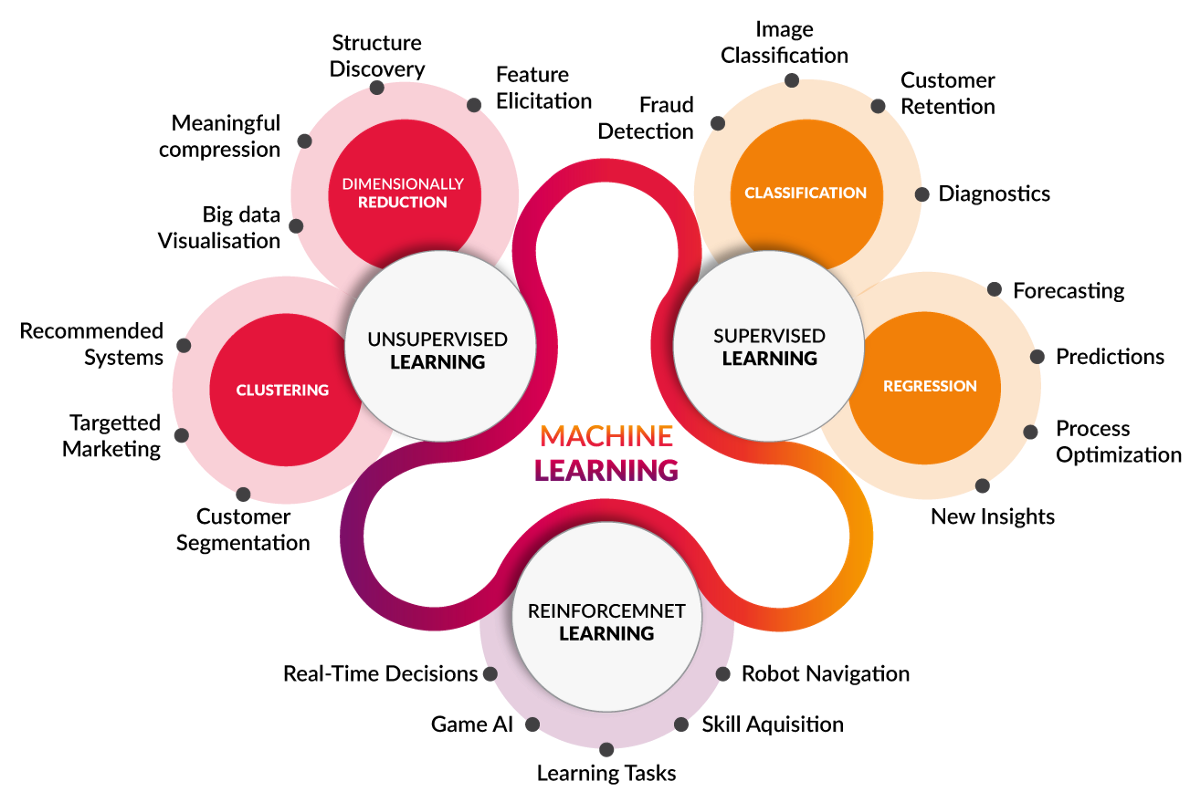
\includegraphics[width=\columnwidth]{images/MachineLearningTypes.png}
	\caption{Machine learning categories}
	\label{fig:mlcategories}
\end{figure}

We will now examine with a bird's eye view what the meaning of supervised and unsupervised learning is, and how they relate to the reinforcement learning methods.  

\subsection{Supervised Learning}

Supervised learning is probably the most widely used of the three main machine learning branches. The word \textit{supervised} comes from the fact that a supervisor, a teacher, is needed within the process. Supervised learning is obtained making an algorithm map input into output data, by first having a large set of training data: these are supervisors of the learning process, since for each given input set of date, the output set is already known. Therefore, the supervised learning is a non-linear function approximation. There are two main areas in which supervised learning is useful: \textit{classification problems} and \textit{regression problems}.
\\
\indent Classification problems are the ones in which the function has to map input data into an output class. For example, an usual classification task would be: given input images of a certain shape and size, tell which pictures contain cats or dogs. The function maps input data into a discrete set of outputs or categories, which come by definition as \textit{labeled} data.
\\
\indent Regression problems concern a more frequent machine learning problem, which is the mapping of input data into a real variable, which is a continuous output. For instance, we can think of a function approximation which, given the size in square meters, distance from the city center, number of rooms and age of a house in Shanghai, can predict its current value. In this case, a set of training data of real house values and their features has to be supplied to the learning algorithm, for predicting prices of houses that had not been seen before.


\subsection{Unsupervised Learning}
Unsupervised learning is learning when only input variables are given, and no outputs are available. The word \textit{unsupervised} comes from the fact that no supervisor is telling how good or bad the algorithm is performing. Therefore, the goal for these methods is to find the underlying structures and patterns in data. Unsupervised learning can be classified into two main subsets, \textit{association} and \textit{clustering}.
\\
\indent Association is about discovering common features in an unlabeled dataset: relationships between different entities can be found by measuring the frequencies of an occurrence in a dataset or with respect to other ones. Association uses probability distributions for measuring the correlation between objects: it is used for instance for giving recommendation on what to add to the checkout basket on a website, knowing behaviors of previous customers.
\\
\indent Clustering is a method for grouping data objects based only on information found in the data describing these objects and their relationship. Cluster analysis's goals are to maximize the similarity within objects in the same group and maximize the difference between objects in different groups: dissimilarities are measured in terms of a distance function and a weight is given to different features in order to provide a clear measure of how much the objects are alike. Clustering has many uses in real-world applications: i.e. the method can be used for identifying fake news, analyzing criminal activities or for personalization and targeting in marketing. 

\subsection{How is Reinforcement Learning different?}

Reinforcement Learning (RL) is a machine learning branch whose main purpose is to make machines learn from experience and make them decide actions to take. It differs from supervised learning since there is no direct need for labeled data: an RL agent could learn from direct interaction with the environment, by just observing the state it is in and a scalar reward (see next Section \ref{sec:elementsRL}). Besides, unlike unsupervised learning, its main purpose is not classification, rather taking decisions; for which unsupervised learning is not suitable.
\\
\indent An important remark about different machine learning methods has to be done though: even if Reinforcement Learning follows a different path with respect to the other machine learning branches, it is usually combined with them for obtaining either better performance or for achieving otherwise impossible results. That is why we will examine also Deep Neural Networks in Chapter \ref{ch:DNN}, which combined with Reinforcement Learning enhance it immensely and give birth to Deep RL, analyzed in Chapter \ref{ch:deeprl}.


\section{Elements of Reinforcement Learning} 
\label{sec:elementsRL}
The problem of reinforcement learning is at the core the interaction of an agent, that can be regarded as our robot, game AI, or even as a human being in a broader sense, which has to select actions on the environment in order to maximize a reward signal over time. In addition to the agent-environment interface which will be further discussed in Section~\ref{sec:MDP}, we can identify four main RL elements:
\begin{itemize}
	\item Policy
	\item Reward signal
	\item Value function
	\item Model
\end{itemize}
\indent The \textit{policy} defines how the agent behaves: in other words, it decides which actions should be selected given the circumstances. For instance, we can imagine Nintendo's arcade game \textit{Super Mario}, in which the hero has to complete levels by avoiding obstacles, beating enemies and jumping across holes in order to reach the flag ending the level or beating an enemy boss. In this scenario, we can consider the policy as the set of actions Mario will take for each situation, like running in a certain direction if there is an incoming foe or jumping with a desired trajectory when trying to overcome a crack in the ground.
\\
\indent The \textit{reward signal} is a scalar value the RL agent wants to maximize: for each time step, a reward signal will be given according to the current state. In the Super Mario example, a positive reward signal could be the score given to each desirable action, like beating an enemy or eating a power-up mushroom. If we want to make Mario avoid dangerous situations that could make him lose a life, we could give him a negative reward: therefore, the agent will try to avoid dangerous situations by trying to maximize the cumulative rewards. Thus, the reward signal is one of the most important tuning parts in a RL algorithm. Rewards can be tuned according to priorities. We could give a +1 reward for each time Mario gets a coin and a much more incisive -10 reward for each time he jumps into a hole; as a result we can make sure our hero will stay away from danger.
\\
\indent Whereas the reward defines what is good in a short time, the \textit{value function} defines what is good in the long run. It gives the value of how much reward the agent can accumulate in the future, starting from a particular state. Making the Mario game analogy, whereas rewards were the immediate scalar values for particular actions, the value of a state is much more farsighted: instead of focusing on a small and immediate reward for beating an insignificant enemy, Mario would rather focus more on a much higher reward in the future, like killing the boss of a level, thus giving up the small immediate reward.
\\
\indent Last but not least, the \textit{model} of an environment is a set of features of the environment itself, useful for easing the computations, predicting value functions and thus making the RL problem much easier to solve. Although models are very useful for planning, it is usual very difficult to craft them: in Super Mario, a model could be labels for each important object in the map and/or providing values of states in advance. Therefore, this one will be called a \textit{model-based} method, as opposed to the more used in RL \textit{model-free} methods, which do not require previous knowledge of the environment. This is because crafting the model itself, given a complicated game or a real-world scenario, could be actually more complex than developing the algorithm necessary for solving the RL problem.


\section{Thesis outline}

The purpose of this thesis is to demonstrate the ability of Reinforcement Learning in being able to control a system without information from any sensors, by just having access to raw visual input. This challenge will first require knowledge of the Reinforcement Learning theory described in Chapter \ref{ch:rl}, in particular about the Q-learning algorithm. In practice, iterative algorithms like Q-learning would need infinite computational power in a continuous state and/or action environment. Therefore, function approximators such as Deep Neural Networks(Chapter \ref{ch:DNN})have to be used for greatly reducing the computational requirements of the problem in mapping the state-action value functions. 
\\
\indent Combining together classical Reinforcement Learning and Deep Neural Networks gives birth to Deep Reinforcement Learning in Chapter \ref{ch:deeprl} which has proven suitable to a wide variety of tasks. After this initial dive into theory we will start in Chapter \ref{ch:CartPole} the real experimental challenge: the vision-based Cartpole balancing implementation in PyTorch using the OpenAI gym package for simulation. In Chapter \ref{ch:conclusion} possible future work that could take this thesis as a starting point will be explored.





\chapter{The Reinforcement Learning problem}

\label{ch:rl}

In this chapter, we will introduce the theoretical bases of reinforcement learning, up to the Q-learning algorithm. This chapter serves as a starting point for the next one, which will regard the extension of the solution proposed here to tackle real world problems.
\section{Markov Decision Processes (MDP)}
\label{sec:MDP}
Before exploring the concept of Markov property and its implications, which are of paramount importance in the reinforcement learning problem, we will first analyze how the agent interacts with its surrounding environment.
\subsection{The Agent-Environment Interface}

The agent-environment interface is a way of better visualizing the RL problem, as in Figure \ref{fig:agentenvironment}\footnote{Source: \href{https://skymind.ai/wiki/deep-reinforcement-learning}{skymind.ai}}.

\begin{figure}[h!]
	\centering
	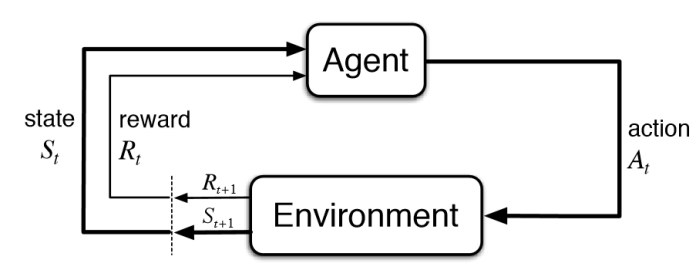
\includegraphics[width=12cm]{images/AgentEnvironment.jpg}
	\caption{The Agent-Environment interface}
	\label{fig:agentenvironment}
\end{figure}
 
The \textit{agent} is the entity acting on the \textit{environment}, that given a $state \ S_t \in \mathcal{S}$ selects one or more $actions \ A_t \in \mathcal{A}$ for interacting with the environment. Our agent then gets feedback from the environment itself: it gets a scalar valued $reward \ R_{t+1} \in \mathcal{R}$, and gets in a new state $S_{t+1} \in \mathcal{S}$. In a \textit{finite} MDP the set of states, actions and rewards ($\mathcal{S},\mathcal{A},\mathcal{R})$ contains a finite number of elements; nonetheless, the problem can be extended in the continuous case. The agent-environment feedback loop repeats over time and it is updated at each time \textit{step}: action selection, state and reward signals are sent only at specific moments in time (t = 0,1,2,3...). The sequence of actions, states and rewards defines a \textit{trajectory} in time that can be described as: 
\begin{equation}
	S_0, A_0, R_1, S_1, A_1, R_2, S_2, A_2, R_3... 
\end{equation}

\subsection{The Markov Property}
\label{sec:markov}
The Markov property is a fundamental concept in RL. The property states that a state $S_t$ is \textit{Markovian} if and only if:
\begin{equation}
	\mathbb{P}[S_{t+1} \,|\, S_t]  = \mathbb{P}[S_{t+1\,} |\, S_1, ..., S_t] 
\end{equation}
The meaning of this equation is that the probability of getting in a state $S_{t+1}$ given the current state $S_t$ is the same probability of getting in that state $S_{t+1}$ given the whole history of states $S_1, ..., S_t$. In other words, the meaning of a process following the Markov property is that future is independent of the past, given the present: hence, this allows us to ignore the history of all the preceding states, in order to decide what to do. Not only theoretically, but also practically speaking this makes the whole process of decision easier.


% MARKOVIANITY / NON EXAMPLES

\subsection{Returns and Rewarding Process}
Given one transition from state $S_t$ to state $S_{t+1}$, we have seen that a single reward is given to the agent. However, what we want to do in RL is to maximize the total sum of rewards $R$ over time. Therefore we define a total \textit{return} $G_t$ as:

\begin{equation}
	G_t  =  R_{t+1} + \gamma R_{t+2} + ...  =  \sum_{k=0}^{\infty}\gamma^k R_{t+k+1}
\end{equation}

Where $\gamma \in [0,1]$ is the \textit{discount factor}. This scalar value is very similar to the one used in economics: we are more interested in money returns which are close in time, but we are less interested in very long-term ones, because these could be just too late for us to benefit. This concept is well described by the sentence: "A dollar today is worth more than a dollar tomorrow". Moreover, discounting makes sense in a biological way since human and animal behavior tends to prefer immediate reward. We can extend this concept to reinforcement learning, by stating that our agent, i.e. Super Mario, will be more interested in getting a payoff as soon as possible, rather than waiting for thousands of time steps for a reward like a coin. Here is how value of $\gamma$ affects our evaluation:

\begin{itemize}
	\item $\gamma$ close to 0: our return evaluation will consider immediate rewards more important than future ones, thus leading to a "myopic" evaluation.
	\item $\gamma$ close to 1: the return function will take very  into account future rewards, thus leading to a "far-sighted" evaluation.
\end{itemize}

Myopic or far-sighted evaluations aside, the discounting process is very important in MDPs since we also avoid an infinite reward, impossible to handle practically speaking.

\subsection{Policies and Value Functions}
A \textit{policy} is the mapping from states to probabilities of selecting each possible action. If an agent at a time $t$ is following a policy $\pi$, then $\pi(a|s)$  describes the probability of taking action $a \in \mathcal{A}$ if it is in the state $s \in \mathcal{S}$:

\begin{equation}
	\pi(a|s)  =  \mathbb{P}[A_t  = a \, |\,  S_t=s]
\end{equation}
\\
\indent In MDPs, we can define the \textit{state-value function} $v_\pi(s)$ as the expected return starting from state $s$ and following policy $\pi$ thereafter:

%WRITE IN APPENDIX WHAT IS THE EXPECTATION


\begin{equation}
	v_\pi(s) \, = \, \mathbb{E}_\pi [G_t \, | \, S_t\,=\,s]
\end{equation}

We can also define an \textit{action-value function} $q_\pi(s,a$), the expected return starting from state $s$, taking action $a$, and then following policy $\pi$:

\begin{equation}
	q_\pi(s,a) = \mathbb{E}_\pi[G_t \, | \, S_t = s, A_t = a]
\end{equation}

\subsection{Bellman Equations}
The \textit{Bellman equations} define how to calculate the state-value functions and action-value functions in an iterative fashion. Since we can express $G_t = R_{t+1} + \gamma G_{t+1}$, then we can decompose the state-value function into immediate reward plus the discounted value of successor state:

\begin{equation}
	v_\pi(s) = \mathbb{E}_\pi[R_{t+1} + \gamma v_\pi (S_{t+1})\, | \, S_t = s]
\end{equation}

The action-value function can be similarly decomposed:

\begin{equation}
	q_\pi(s,a) = \mathbb{E}_\pi[R_{t+1} + \gamma v_\pi (S_{t+1},A_{t+1})\, | \, S_t = s, A_t = a]
\end{equation}

\subsection{Optimality Conditions}
The ultimate goal of RL is to obtain a policy which is \textit{optimal} in the sense that it is better in decision making than all other policies. We define the \textit{optimal state-value function} as:
\begin{equation}
	v_*(s) = \max_\pi v_\pi(s)
\end{equation}
In a similar way, the \textit{optimal action-value function} is defined as:
\begin{equation}
	q_*(s,a) = \max_\pi q_\pi (s,a)
\end{equation}
We define an ordering over policies: a policy is greater than another one if the values of all of its states are greater than those of the second one or that $\pi \geq \pi'$ if $v_\pi(s) \geq v_{\pi'}(s), \forall s$. For any Markov Decision Process:

\begin{itemize}
	\item An optimal policy $\pi_*$ such that it is better or equal to all other policies $\pi_* \geq \pi, \forall \pi$ exists
	\item All optimal policies achieve the optimal value function, $v_{\pi_*}(s)=v_*(s)$
	\item All optimal policies achieve the optimal action-value function, $q_{\pi_*}(s,a)=q_*(s,a)$.
\end{itemize}

Since the goal is finding the optimal policy, it can be found by maximizing over $q_*(s,a)$,

\begin{equation}
	\pi_*(a|s) = \begin{cases}
	1, & \text{if $a = \argmax_{a \in \mathcal{A}} \, q_*(s,a)$}\\
	0, & \text{otherwise}.
	\end{cases}
\end{equation}

This means that if the probability of the policy of selecting the best possible action is 1 . In order to find a solution for the Bellman Optimality Equation, which is not linear, many iterative solution methods have been developed. 

\subsection{Exploration and Exploitation}
\label{sec:explorationExploitation}
One of the most important problems in Reinforcement Learning, which does not have a single best answer, is the exploration and exploitation one. So far, we stated that the best way of choosing actions is to always select the action which seems optimal because it results in the highest reward: this is the \textit{exploitation} since the agent exploits what it thinks is the optimal solution.
\\
\indent However, during the learning process, it may be extremely important for the agent to sometimes choose the sub-optimal action because this may prevent it to get stuck in some local optimum. This is the process of \textit{exploration}. For example, if Super Mario has to reach the end flag of a level, maybe he knows the optimal path to get there in the least time possible. However, if he always did so, then he would never discover other possible better solutions like going down a pipe and earning a Star Coin first, or maybe just jumping onto a block and getting a tasty power-up. 
\\
\indent A widely used solution, called the \textit{$\varepsilon$-greedy} action selection, is not to always take the seemingly best action, but to take it with probability $1 - \varepsilon$, and to take a random action with probability $\varepsilon$:

\begin{equation}
\pi(a|s) = \begin{cases}
1 - \varepsilon, & \text{if $a = \argmax_{a \in \mathcal{A}} \, q_*(s,a)$}\\
\varepsilon, & \text{a random action}.
\end{cases}
\end{equation}

\section{Dynamic Programming}
One of the most important contributions to the RL research field is the Dynamic Programming (DP)\cite{bertsekas1995dynamic} approach. DP is a method for solving complex problems, by breaking them down into sub-problems, solving their sub-problems, and finally combining solutions to the sub-problems to solve the overall complex problem. Dynamic programming is a very general method for problems which have two main properties:

\begin{itemize}
		\item \textit{Optimal substructure}: if an optimal solution of the problem can be constructed from optimal solutions of its sub-problems. For example, if a car has to find the shortest path to a certain destination, then what can be done is to first find the shortest path a midpoint in the route, and then find the shortest path from the midpoint to the final destination.
		\item \textit{Overlapping problems}: the sub-problems which occur once, will occur again and again. In the car example, we broke down the problem into two sub-problems: getting from the starting point to a midpoint, and from the midpoint to the end. This solution will help to solve the sub-problem of how to get from another point to the final destination: solutions can thus be cached and reused.
\end{itemize}

As it turns out, Markov Decision Processes satisfy both the aforementioned properties. The Bellman Equation results in a recursive decomposition: it breaks down the calculation in two parts, the optimal behavior for one step followed by the optimal behavior after that step. The overlapping problems solution in MDPs is given by the value function: it is like a cache of the information we have collected about the MDP. In the car example, after figuring out the optimal path to the final destination, that information is store: when we need that datum for a similar path, we will have already computed it and we will not need to recompute it.

\subsection{Dynamic Programming Shortcomings}
Although it introduces useful tools for solving reinforcement learning problems, DP has important shortcomings. Firstly, DP methods are \textit{model based} and require a complete knowledge of the environment, such as transition probabilities and rewards. Secondly, they suffer from the \textit{curse of dimensionality} since, having to perform a complete backup of all states and transition, increasing the state and action spaces dimensions will exponentially increase the calculations required for solving the problem; which becomes impossible if the dimensionality approaches infinity in continuous spaces.

\subsection{Generalized Policy Iteration}
\label{sec:gpi}
Before going to explore the Monte Carlo methods and following algorithms that try to solve the curse of dimensionality, we need to introduce the Generalized Policy Iteration (GPI), which is an iterative scheme composed of two steps:
\begin{itemize}
	\item \textit{Policy evaluation step}: an approximation of the value function based on the current policy is created .
	\item \textit{Policy improvement step}: the policy is improved with respect to the current value function, by acting greedily on it.
\end{itemize}

This process will always converge, after a number of iterations, to the optimal policy $\pi_*$.


\section{Monte Carlo Methods}
The idea behind Monte Carlo (MC)\cite{metropolis1949monte} methods was derived from the same-name casino: finding out a way of solving a problem by using a major random component. Monte Carlo methods work on the concept of GPI of Section \ref{sec:gpi}: they learn value functions from direct interaction with the environment by means of episodes of experience; performing random rollouts on the system and by updating the accumulation of rewards and the distribution of states encountered at the end of the episode. The current policy is then estimated by making it directly greedy with respect to the current value function. Using these two steps iteratively, it can be shown that the algorithm converges to the optimal value function and policy.
\\
\indent Since they do not require a model, Monte Carlo methods are \textit{model-free} ones, thus they have a major advantage with respect to the model-based Dynamic Programming. A simple every-visit MC method calculating the value of a state is:

\begin{equation}
	V(S_t) \gets V(S_t) + \alpha[G_t - V(S_t)]
	\label{eq:MC}
\end{equation}

where $G_t$ is the actual return at time $t$, and $\alpha \in (0,1]$ is the \textit{learning rate}, a step-size parameter indicating how much we shift our estimate $V(S_t)$ towards a more realistic value based on the calculation of the actual return. As it can be noticed, the value of $G_t$ can only be computed at the end of the episode, so value updates will happen only at that moment.
\\
\indent Although MC methods are relatively simple and straightforward in their implementation, they require a large number of iterations for their convergence and suffer from a large variance in their value function estimation: hence, they cannot be considered efficient for the majority of RL purposes. Nonetheless, they are conceptually very important in the development of more complex algorithms.

\section{Temporal Difference Methods}

Temporal Difference (TD) methods combine concepts from both Dynamic Programming and Monte Carlo methods in order to avoid some of the shortcomings of both methods. TD builds on the same idea of Generalized Policy Iteration, but differs from Monte Carlo in the policy evaluation step. Whereas MC methods use the total accumulated reward $G_t$ to make predictions and have to wait until the end of the episode, as seen in Equation \ref{eq:MC}, TD methods only need to wait until the next time step for updating. The simplest TD method makes the update:

\begin{equation}
V(S_t) \gets V(S_t) + \alpha[R_{t+1} + \gamma V(S_{t+1}) - V(S_t)]
\label{eq:TD}
\end{equation}

immediately on transition $S_{t+1}$ and receiving $R_{t+1}$, and does not have to wait until the end of the episode knowing a better estimate of our state value. The quantity in the brackets can be seen as a sort of error since it is the difference between $R_{t+1} + V(S_{t+1})$, the new estimate, and $V(S_t)$, the old estimate. This quantity called \textit{TD error} is important in many reinforcement learning algorithms:

\begin{equation}
	\delta _t \doteq R_{t+1} + \gamma V(S_{t+1}) - V(S_t)
\end{equation}
\\
\indent Like in Monte Carlo methods, TD learns directly from episodes of experience, and being \textit{model-free}, it has a major advantage in environments where MDP transitions and rewards are not known. However, Temporal Difference methods have a major advantage over MC ones: they can learn by \textit{incomplete} sequences of episodes, by \textit{bootstrapping}. Bootstrapping is the idea of updating a guess, $V(S_t)$, towards a guess,  $R_{t+1} + \gamma V(S_{t+1})$: this way, we do not have to wait until the end of an episode.
\\
\indent For example, suppose you want to drive home and the navigation algorithm tells you will take 30 minutes to get there. But then, after 5 minutes, you are stuck in a traffic jam, which will add another 30 minutes to your commuting. A Monte Carlo algorithm would have to wait until you have reached home, finishing your "episode", to update its estimate. In contrast, a TD one would update the estimated time to arrival in real time, telling that you will have another 55 minutes driving home. As a result, the latter method is much more useful in this real life application.
\\
\indent Two TD algorithms which have been widely used to solve RL problems are \textit{SARSA} and \textit{Q-Learning} will be explored in the next chapters.

\subsection{SARSA}

SARSA (\textit{State-Action-Reward-State-Action}) is an on-policy temporal difference algorithm which tries to learn an action value function, instead of the value one. The policy evaluation step uses the TD error for the action value function, which is similar to the value function. SARSA is an \textit{on-policy} learner since it learns the value function of the current policy; in contrast, an \textit{off-policy} learner learns the value functions of the optimal policy while following another one.
\\
\indent The idea behind SARSA is choosing actions with an \textit{$\varepsilon$-greedy} policy and then updating the value of the action value function $Q(s_t, a_t)$, which is the value of being in state $s$ at time $t$ and taking action $a$, after observing the reward $r_{t}$ and the state we reach at time $t+1$,  $s_{t+1}$. The algorithm is summarized below in pseudo code:

\begin{algorithm}
	\caption{SARSA}
	\SetAlgoLined
	\DontPrintSemicolon
	Initialize $Q(s,a)$ randomly\;
	\Repeat{terminated}{
	Observe initial state $s_1$\;
	\For{t=1: T}{
	Select an action $a_1$ using policy derived from Q (e.g. $\varepsilon$-greedy)\;
	Carry out action $a_t$\;
	Observe reward $r_t$ and new state $s_{t+1}$ \;
	Update Q using 
	% MATCH SYNTAXXX!! LIKE s'
	\begin{equation} 
		Q(s_t, a_t) \gets Q(s_t,a_t) + \alpha[r +  \gamma Q(s_{t+1}, a_{t+1}) - Q(s_t,a_t)]		
	\end{equation}
}
}
\end{algorithm}



\subsection{Q-Learning}
\label{sec:qlearning}

Q-Learning\cite{watkins1992q} is one of the simplest but still quite efficient algorithms, and one of the earliest breakthroughs in Reinforcement Learning. It is an off-policy TD control algorithm which is similar to SARSA but differs in the way the action value funtion $Q(s_t, a_t)$ is updated (see Algorithm \ref{alg:Qlearning}.)

\begin{algorithm}[H]
	\label{alg:Qlearning}
	\caption{Q-learning}
	\SetAlgoLined
	\DontPrintSemicolon
	Initialize $Q(s,a)$ randomly\;
	\Repeat{terminated}{
		Observe initial state $s_1$\;
		\For{t=1: T}{
			Select an action $a_1$ using policy derived from Q (e.g. $\varepsilon$-greedy)\;
			Carry out action $a_t$\;
			Observe reward $r_t$ and new state $s_{t+1}$\;
			Update Q using 
			% MATCH SYNTAXXX!! LIKE s'
			\begin{equation} 
			Q(s_t, a_t) \gets Q(s_t,a_t) + \alpha[r + \max_a \gamma Q(s', a) - Q(s_t,a_t)]	
			\label{eq:Qlearning}	
			\end{equation}
		}
	}
\end{algorithm}

As we can notice in Equation \ref{eq:Qlearning}, the most important difference between SARSA and Q-Learning is the update rule; while in the former the action value function is updated based on the current policy, Q-Learning updates $Q(s_t, a_t)$ directly greedily follow another policy that is, for example, an $\varepsilon$-greedy one.
\\
\indent These algorithms have proven very efficient in low dimensional state and action spaces. However, for real life applications, the number of states and/or actions greatly exceeds what we can consider of low dimensionality. Therefore, we will need further tweaking methods for an actual implementation of these algorithms.



\chapter{Deep Neural Networks}
\label{ch:DNN}
\section{Why Neural Networks?}

The methods discussed up to now are called \textit{tabular methods}. This means that we are actually saving values of the value function is in a table, which is a very easy way. However, tabular methods are usable only in very low dimensionality problems, otherwise, the amount of memory required to store all the data would be extremely large. Additionally, when trying to look up for a value of a particular state, it will require an entire sweep of the table which is computationally expensive. Moreover, if the state space is continuous, a tabular format is impossible. To overcome this problem, \textit{function approximators} are used to store value functions.
\\
\indent Many function approximation algorithms have been developed over the years, but one of the most recent breakthroughs in Machine Learning was the development of \textit{Deep Neural Networks (DNNs)}. These methods have given a surge in the field of Reinforcement Learning algorithms, and have paved the way for successfully carrying out tasks that were once considered impossible, such as the AlphaGo project\cite{silver2017mastering}.

\section{Building Units}

	Artificial neural networks are inspired and loosely modeled after how the human brain works. The human brain is a complex web of interconnected neurons, its building units, which is capable of extracting critical information from the inputs and producing a corresponding output (signal). In a similar way, a Deep Neural Network consists of a set of interconnected neurons, arranged in layers, where each neuron takes some real value input and gives a real valued output. 

\begin{figure}
	\centering
	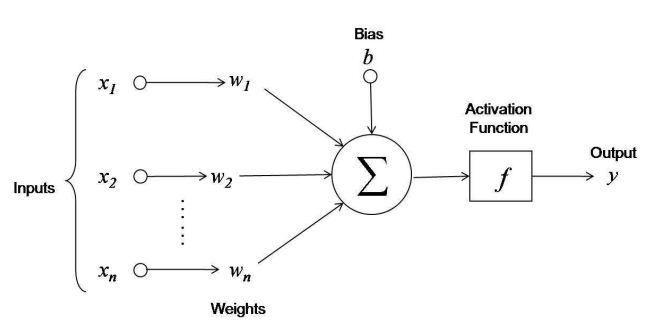
\includegraphics[width=10cm]{images/NeuronDiagram}
	\caption{An artificial neuron}
	\label{fig:neuron}
	
% NOTE: WE CAN INSERT JUST A LINK OF CITATION TO THE IMAGE! AS IN THE LEO THESIS

\end{figure}

\subsection{Artificial Neuron}
Figure \ref{fig:neuron}\footnote{\href{https://medium.com/@jayeshbahire/the-artificial-neural-networks-handbook-part-4-d2087d1f583e}{Source: medium.com}} shows an artificial neuron. The neuron takes as input a vector of inputs $x = [x_1, x_2, ..., x_n]$ and calculates a weighted sum of the inputs, with the neuron \textit{weights} denoted by the vector $w_i = [w_{i,1}, w_{i,n}, ..., w_{i,n}]$, which is actually the $i_{th}$ row of a weight matrix. The weighted sum is then added to a \text{bias} term, $b$, and then is passed through an \textit{activation function}, $f$, which produces the output of the neuron. Our  complete equation for a single neuron can be written as:


\begin{equation}
	\label{eq:neuron}
	y_i = f(\sum_{j} x_j w_{i,j} + b_i)
\end{equation}

where $j$ is the number of inputs to the neuron, and $i$ represents the $i_{th}$ layer of neurons of the DNN.
\\
\indent What we can see here is that a single neuron carries indeed a non-linear function, and the interconnecting of many neurons gives the DNN a great complexity, but it also enables it to be a very powerful tool. Indeed, even if the single neuron is modeled after the biological one, since biological neurons have thousands of connections with neighboring ones and also have the ability of destroying and creating connections, they are still far more efficient than even state-of-the-art Deep Neural Networks as of writing time.

\subsection{Activation Functions}
\label{subsec:ActivationFunctions}
The activation function introduces non-linearity to the output of a neuron: this is extremely important for the network in order to learn non-linear representations from the training data. In literature, a number of activation functions have been introduced, like \textit{sigmoid}, \textit{hyperbolic tangent}, and \textit{rectified linear unit}. These commonly used activation functions are explained below:

\begin{itemize}
	\item Sigmoid: 
	\begin{equation}
		f(x) = \dfrac{1}{1 + e^{-x}}	\end{equation}
\end{itemize} 

\begin{itemize}
	\item Hyperbolic Tangent: 
	\begin{equation}
	f(x) = \dfrac{e^x - e^{-x}}{e^x + e^{-x}}	\end{equation}
\end{itemize} 

\begin{itemize}
	\item Rectified Linear Unit (ReLu)\cite{nair2010rectified}: 
	\begin{equation}
	f(x) = \max(0,x)
	\label{eq:ReLu}	
	\end{equation}
\end{itemize} 

 Since ReLu does not suffer from saturation as compared to the other two functions discussed above, it is the one providing the best performance over a wide variety of tasks.

\section{Feed Forward Networks}
\label{sec:feedforward}
The most common architecture used in DNN is the \textit{Feed-Forward} neural networks. Figure \ref{fig:feedforward}\footnote{\href{http://cse22-iiith.vlabs.ac.in/exp4/index.html}{Source: vlabs.ac.in}} shows an example of this architecture.

\begin{figure}[h]
	\centering
	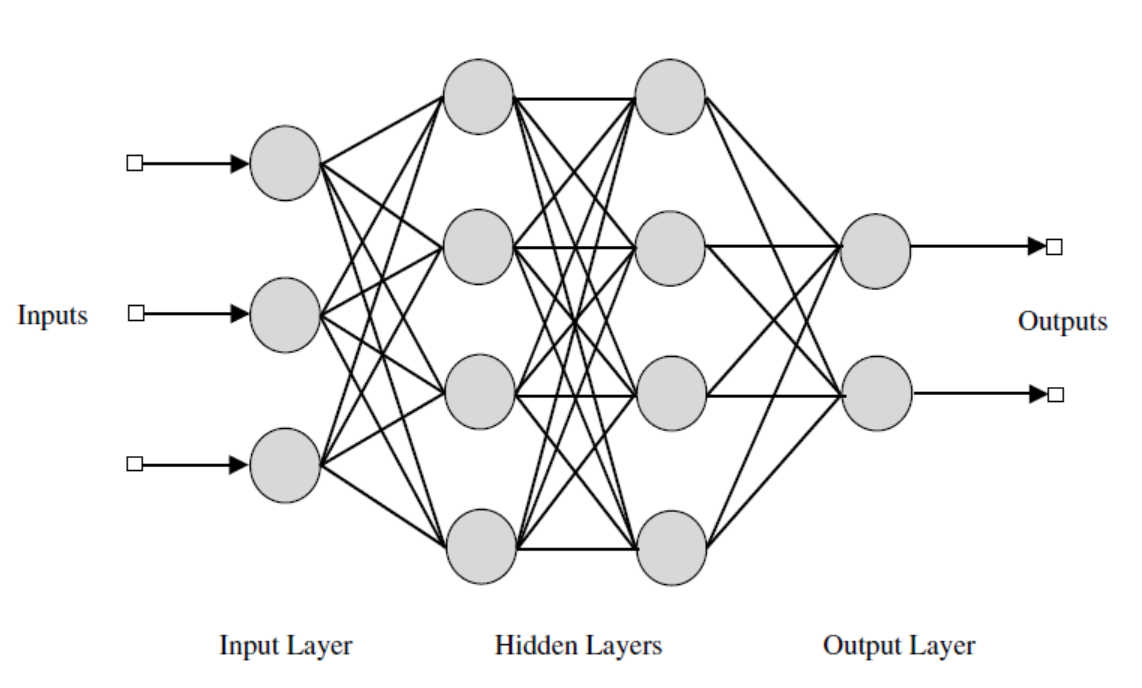
\includegraphics[width=10cm]{images/FeedForward}
	\caption{A Feed Forward neural network with two hidden layers}
	\label{fig:feedforward}
	% NOTE: WE CAN INSERT JUST A LINK OF CITATION TO THE IMAGE! AS IN THE LEO THESIS
	
\end{figure}

In this framework, neurons are arranged in three kinds of layers:

\begin{itemize}
	\item One \textit {input layer}: where the flow of information begins, this is the layer taking the raw input: therefore, the number of input neurons will be equal to the number of input features.
	\item One or more \textit{hidden layers}: these may have a variable number of neurons, and they serve as an intermediate stage between inputs and outputs making the neural network able to predict more complex outputs. \textit{Deep} NNs are called like this because of the hidden layers.
	\item One \textit{output layer}: where the flow of information ends, this is the layer predicting the outputs: neuron number will be equal to the number of output features.
\end{itemize}

Each single neuron in the different layers performs the computation shown in Equation \ref{eq:neuron}.

\subsection{Training the Network}
\label{subsec:traininnet}

The weights of the neural network are trained with a technique known as \textit{backpropagation}. The idea of this approach is the initialization of the network with random weights and then the calculation the output for a given input. Initially, since the network has not been trained yet, it will produce a random output. The error between the generated output and the actual output is used to update the weights using a gradient descent algorithm: the error function will gradually be minimized, so will the error between the generated and the actual output. This way, we will have successfully approximated the function we have trained the network on. Since the weights are first updated on the output layer and then propagated back into the network, the technique is known as backpropagation.
\\
\indent In recent years, a number of new training techniques have been introduced. One of the most popular choices has been the \textit{stochastic gradient descent}, but new improved versions have been successfully developed, like \textit{ADAM (A Method for Stochastic Optimization)}\cite{kingma2014adam}. These methods have advantages over using the traditional gradient descent because they can vary learning rates based on the distribution of training data. This is very convenient since they reduce the need for careful choice of the learning rate, which in turn allows a faster convergence of the algorithm.

\subsection{Underfitting and Overfitting}
\label{sec:overfitting}

Two of the most common problems which can be encountered in neural networks are underfitting and overfitting, shown in Figure \ref{fig:fitting}\footnote{Source: \href{https://medium.com/greyatom/what-is-underfitting-and-overfitting-in-machine-learning-and-how-to-deal-with-it-6803a989c76}{medium.com}}.

\begin{figure}[h!]
	\centering
	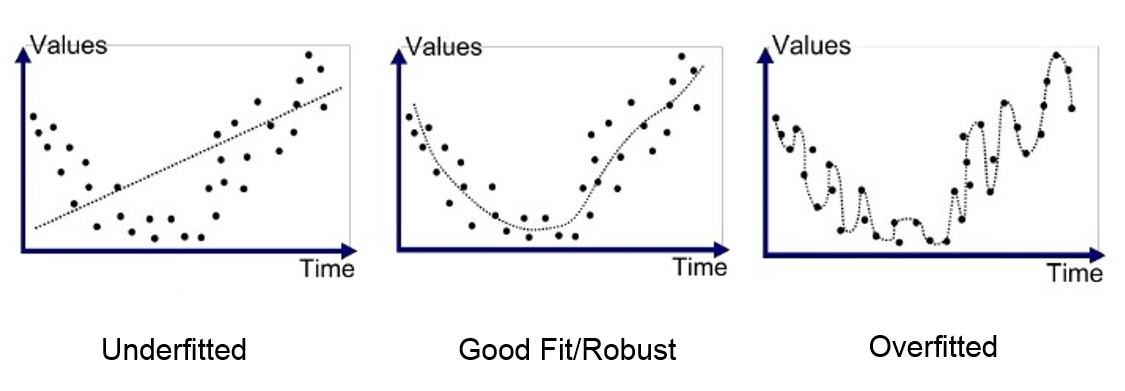
\includegraphics[width=10cm]{images/UnderOverFitting.png}
	\caption{Examples of underfitted, good fit and overfitted networks}
	%https://cdn-images-1.medium.com/max/1200/1*_7OPgojau8hkiPUiHoGK_w.png
	\label{fig:fitting}
\end{figure}

\textit{Underfitting} is a situation in which our network cannot approximate the function in a good way; in other words, the model is too simple for describing a complex data distribution. One way of reducing this problem is to increase the degree of the polynomial describing our function, so that it will approximate the function shape in a better way.
\\
\indent \textit{Overfitting} is, in a sense, the opposite of underfitting: it is a situation in which the network's model approximates the function in a "too good to be true" way. In this case the problem is that the model learned cannot generalize to new data, since it was trained too well on the training data. To overcome this problem, there are a number of solutions, such as \textit{Regularization} and \textit{Dropout}.

\section{Convolutional Neural Networks}

Convolutional Neural Networks (CNN) are an evolution of Feed Forward NNs which are able to deal with inputs of very high dimensionality. One of the most important uses for CNNs is image recognition, because indeed images are high dimensionality tensors. For example, a very simple square Grayscale image of 28 pixels is a 28x28x1 tensor, and if we had to flatten it for feeding to a classical feed forward network, the number of neurons required would be simply too high for a network to be efficient. Therefore, CNNs were developed for dealing with such problems.

\subsection{CNN Architecture}
Figure \ref{fig:CNN}\footnote{Source: \href{https://towardsdatascience.com/a-comprehensive-guide-to-convolutional-neural-networks-the-eli5-way-3bd2b1164a53}{Source: towardsdatascience.com}} shows a simple CNN for recognizing hand-written digits, which is used frequently for a first approach in learning neural networks. Among with some building blocks we have already seen, these are the main architecture component for a Convolutional Neural Network:

\begin{figure}[h]
	\centering
	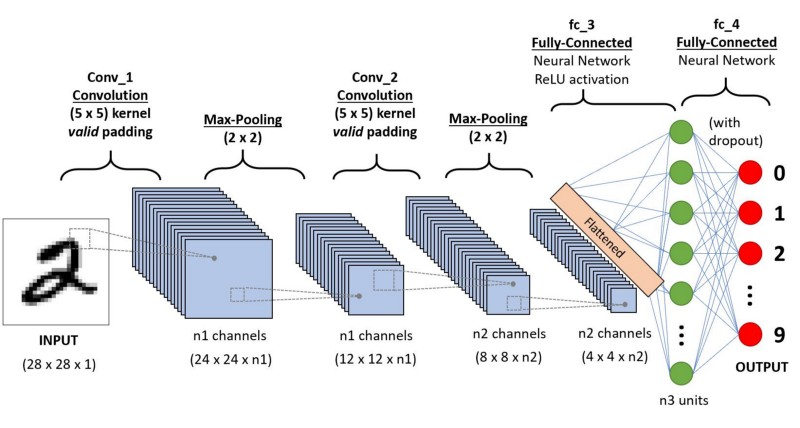
\includegraphics[width=11cm]{images/CNN.jpeg}
	%https://towardsdatascience.com/a-comprehensive-guide-to-convolutional-neural-networks-the-eli5-way-3bd2b1164a53
	\caption{A CNN for recognizing hand-written digits}
	\label{fig:CNN}
\end{figure}

%ASK FOR HOW TO DEAL WITH THIS PART

\begin{itemize}
	\item \textit{Convolutional layers}: Convolutional layers are the core building blocks of CNNs. They build up on the idea of fully connected layers we have seen before, with the main difference being they are much more computationally efficient, especially for image processing. The layers parameters consist of a set of learnable \textit{filters} (also called \textit{kernels}): they are \textit{convolved} across the width and height of the input volume (the filter is forward passed above each of the image pixels), computing the dot product between the parameters of the filter and the input, producing a 2-dimensional activation map of that filter. 
	\\
	\indent The network works by learning filters activating when they detect specific types of features at some spatial position for the input.
	\item \textit{Pooling layers}: These are another type of fundamental building blocks in CNN. A pooling layer is a form of non-linear down-sampling: it is able to reduce the memory usage, the amount of computation in the network, and it is also useful for controlling overfitting. It is common to insert a pooling layer among two successive convolutional layers. 
	\\
	\indent A common type of these layers is the \textit{max pooling}: it basically splits an image into a series of squares, each made of a number of pixels, and then downsamples it by taking the maximum of each group of pixels. For instance, if we have a 24x24 layer, a possible max pooling layer would divide it into 2x2 squares, take the maximum among them, and then producing a final layer of 12x12 made up of the maximums. This greatly reduces the computational requirements of the architecture.
	%\item \textit{Flattening}:
	
	\item \textit{Activation layers}: These layers apply non-linearities in the neural network. As we have already seen in Section \ref{subsec:ActivationFunctions} , a non-saturating activation function which has proven to be very efficient is the ReLu\cite{nair2010rectified} (Equation \ref{eq:ReLu}).
	 
	\item  \textit{Fully connected layers}: These layers carry out the high-level reasoning in the neural network, after several convolutional and pooling layers. Neurons in a fully connected layer have connections to all activations in the previous layer, as seen in the Feed Forward networks (Section \ref{sec:feedforward}). The fully connected layer is then connected to the output layer. In this section is possible to apply well known feed forward NNs techniques, for instance in preventing overfitting such as the \textit{dropout}\cite{srivastava2014dropout} technique.
\end{itemize}

\subsection{Applications}

Convolutional Neural Networks have been used for several years in many fields. They have proven to be a great tool in \textit{image recognition} systems, in which they find the most important application to date. 
\\
\indent Another frequently used implementation for CNNs is \textit{video classification}, in which the networks were found to be very efficient. The techniques basically implement image recognition to video inputs which are indeed a stream of frames one after another. 
\\
\indent \textit{Signal elaboration} is a research field in which CNNs are being used more and more. The vast complexity of the signal domain is an ideal case to be handled by this NN architecture, given its ability to decrease the need of overly-powerful computers.
\\
\indent For the purposes outlined in this thesis, an important use for Convolutional Neural Networks is the \textit{Reinforcement Learning} field. Aside of the early CNNs breakthroughs in the checkers game and the more recent development with AlphaGo\footnote{Source: \href{https://deepmind.com/research/alphago/}{deepmind.com}}, a direct implementation of CNNs along with Q-Learning are the Deep Q-Networks (DQNs, Section \ref{sec:DQN}), which have proven reliable in learning directly from high-dimensional sensory inputs.

\chapter{Deep Reinforcement Learning}
\label{ch:deeprl}

\section{Introduction}
As we have seen in Deep Neural Networks (Chapter \ref{ch:DNN}), a major improvement for the efficiency of RL algorithms is the introduction of function approximators which are able to generalize functions using much less data than a tabular method would require. A function approximator approximates a generic function $f(x)$ to a $f'(x;\theta) \approx f(x)$, where $\theta$ are the weights of the neural network.

% THETA OR w FOR WEIGHT?? DECIDE

\section{Deep Q-Learning}

\label{sec:DQN}
Q-Learning (Section \ref{sec:qlearning}) has been a widely used algorithm for model-free reinforcement learning. Although this method is relatively simple and it seemingly can not handle high-dimensionality problems, it was shown in the Atari 2600 paper\cite{mnih2013playing} that the implementation of Q-Learning along with Deep Neural Networks, called \textit{Deep Q-Learning (DQN)}, can indeed handle problems with a very high state dimensionality. The DQN algorithm was able to show human level performance on seven Atari 2600 games using only raw image pixels as input. Given the importance of the aforementioned paper in the Deep Reinforcement Learning field, we will use the same notation here.
\\
\indent The non-linear function approximator, in this case neural network, will have the task of estimating the action-value function, $Q(s,a; \theta) \approx Q*(s,a)$. For our purposes, $\theta$ will denote the set of weights of the network, which we will refer to as Q-network. A Q-network can be trained by minimizing a sequence of loss functions $L_i(\theta_i)$ changing at each iteration i,

\begin{equation}
	L_i(\theta_i) = \mathbb{E}_{s,a \sim \rho(\cdot)}[\left(y_i - Q(s,a;\theta_i)\right)^2],
	\label{eq:lossfunction}
\end{equation}

where $y_i = \mathbb{E}_{s' \sim \mathcal{E}} [r + \gamma \max_{a'}Q(s', \theta_{i-1}) | s,a]$ is the target for iteration $i$, $\rho(s,a)$ is a probability distribution over sequences $s$ and actions $a$ that we refer to as the \textit{behavior distribution}, and $\mathcal{E}$ refers to the environment. The parameters from the previous iteration $\theta_{i-1}$ are kept fixed when optimizing the loss function $L_i(\theta_i)$. The targets depend on the network weights: for this reason, it differs from classical weights used in supervised learning, which are fixed before learning itself begins. 
\\
\indent Since we want to minimize the loss function for obtaining a better fit of the networks with respect to the real action value function, we want to compute the gradient with respect to the weights:

\begin{equation}
	\nabla_{\theta_i}L_i (\theta_i) = \mathbb{E}_{s,a \sim \rho(\cdot); s' \sim \mathcal(E)} [(r + \gamma \max_{a'} Q (s', a'; \theta_{i-1}) -  Q(s,a; \theta_i)) \nabla_{\theta_i} Q(s,a; \theta_i)]
	\label{eq:gradientloss}
\end{equation}

The loss function is then minimized as explained in Section \ref{subsec:traininnet} by either using stochastic gradient descent or more sophisticated methods like ADAM. The behavior policy is $\epsilon$-greedy for ensuring sufficient exploration.
\\
\indent What makes the algorithm work is a technique known as \textit{experience replay}\cite{schaul2015prioritized}, by which we store the agent's experiences (also referred to as transitions) at each time-step, $e_t = (s_t, a_t, r_t, s_{t+1})$, in a data set $ \mathcal{D} = (e_1, ..., e_N)$, pooled over many episodes into a \textit{replay memory}. In the inner loop of our algorithm we apply Q-Learning updates, or mini-batch updates, to samples of experience, $e \sim \mathcal{D}$, picked up randomly from the pool of stored samples. After performing experience replay, the agent executes an action according to an $\epsilon$-greedy policy. Deep Q-Learning with experience replay is written in pseudo-code in Algorithm \ref{alg:DQN}.
\begin{algorithm}[h]
	\caption{Deep Q-Learning with Experience Replay}
	\label{alg:DQN}
	\SetAlgoLined
	\DontPrintSemicolon
	Initialize replay memory $\mathcal{D}$ \;
	Initialize action value function Q with random weights \;
	\Repeat{terminated}{
		Observe initial state $s_1$\;
		\For{t=1: T}{
			Select an action $a_1$ using policy derived from Q (e.g. $\epsilon$-greedy)\;
			Carry out action $a_t$\;
			Observe reward $r_t$ and new state $s_{t+1}$\;
			Store transition $(s_t, a_t, r_t, s_{t+1})$ in replay buffer $\mathcal{D}$\;
			Sample random transitions $(s_j, a_j, r_j, s_{j+1})$ from $\mathcal{D}$\;
			Calculate target for each transition \;
			% MATCH SYNTAXXX!! LIKE s'
			
			\begin{equation}
			\text{Set } y_i = \begin{cases}
			r_j & \text{if } s_{j+1} \text{ is terminal}\\
			r_j + \gamma \max_{a'} Q(s_{j+1},a';\theta) & \text{if } s_{j+1} \text{ is non-terminal}			
			\end{cases}
			\end{equation}
			
			Train the Q network on $(y_j - Q(s_j, a_j; \theta))^2$ using Equation \ref{eq:gradientloss}
		}
	}
\end{algorithm}
\\
\indent Deep Q-Learning has several advantages by using experience replay. Firstly, since each step of experience is potentially used in many weight updates, we have a greater data efficiency. Secondly, randomizing the samples allows for improved efficiency and reduces the updates variance, given that learning directly from consecutive samples of experience is inefficient due to the strong correlations between the samples. Thirdly, by learning off-policy we may be able to avoid dangerous unwanted feedback loops. For example, if we did train on-policy, if the maximizing action were to move on the left then the training samples would be dominated by samples from the left-hand side; if the maximizing action were the opposite one on the right, the same would happen with the right-hand side samples. This behavior could lead to unwanted outcomes, like getting stuck in a poor local minimum, or even catastrophically diverge. Thus, by using the off-policy experience replay we are able to smooth out learning and to avoid oscillation or divergence in the parameters.

\subsection{DQN shortcomings}
Even if the algorithm demonstrated robustness in the Atari 2600 games, there are a few issues it is not able to solve. The algorithm only stores the last $N$ experience tuples in the replay memory, and samples uniformly at random from $\mathcal{D}$ when performing updates. Firstly, the approach is in some respects limited since the memory buffer treats all transitions equally and does not address important ones; secondly, due to the finite memory size $N$, the algorithm always overwrites with the most recent transitions. Moreover, the uniform sampling gives equal importance to all transitions in the replay memory; as stated in the Atari 2600 paper\cite{mnih2013playing}, a more sophisticated strategy might address these problems, for example by prioritizing important transitions.



\chapter{Cart-Pole Balancing with Visual Input}
\label{ch:CartPole}

After exploring the most important Deep Reinforcement Learning algorithms, this chapter shows the empirical results for the vision-based control of the Cart-pole balancing problem.
\\
\indent One question the reader may ask could be: why choosing the \textit{CartPole} problem from OpenAI Gym in the first place? 

\section{Why Cart-Pole Balancing?}
\label{sec:whyCartPole}

Balancing of a Cart and Pole has been already achieved and its control system may be even based on well-known and robust techniques such as with Proportional-Integral-Derivative (PID) controllers. The difference with these control methods and RL is that the former require a complete model of the environment: all the dynamics must be known and analytical/numerical methods have to be found in order to solve the problem. In other words, sensors have to be put on a system in order to be able to control it, which could not be the case for applications in which sensors cannot be placed directly on the system or would have a negative impact on its dynamics. Besides, a classical controller such as a PID cannot be used when we are required to control a too complex environment, such as an agent in a computer game: in this case, the only ways to control this game AI would be either to hard-code it (for instance, "AI" from the famous Atari 2600's game \textit{Pong} used a simple code to just follow the ball trajectory), with the issues being hard work and impossibility of the game's bot to improve over time. Moreover, building a game AI via hard-coding for complex tasks highly inefficient and almost impossible.
\\
\indent DRL, on the other hand, has shown amazing results in either computer game agents or for more difficult tasks such as making a robot learn to walk or grasp objects. A famous paper among the DRL researchers, \textit{Playing Atari with Deep Reinforcement Learning}, demonstrated the ability of the DQN algorithm to solve complex tasks such as achieving super-human performance in most of the Atari 2600's games by using only batches of video frames.
\\
\indent
Because of the proven abilities of Deep Q-Networks to deal with high-dimensional states with a discrete number of actions, we chose DQN to deal with the CartPole problem. The choice of this task was due to it being relatively simple and used as a test benchmark of control algorithms, yet challenging since in our case no information about velocities and positions of the system are give.
\\
\indent
Our goal will then be to answer the following question: can the DQN algorithm solve the CartPole, using as inputs only video frames of the game being run?

\section{Experimental Setup and Tools} 

In this section, the settings and tools used for conducting the experiments will be discussed in order to provide the reader with a repeatable experimental setup.

\subsection{Hardware and Software}
\label{sec:hardwaresoftware}
As regards the Hardware, we used in our experiments a laptop with medium specs: a dual-core CPU (i7-7500U), 16GB of DDR4 RAM, and a GTX 950M Nvidia GeForce GPU with 2GB dedicated video memory. The requirements for the CartPole task do not require a top-level machine learning setup, although it is very power-demanding during training.
\\
\indent The experiments were run using Ubuntu 18.04 operating system. The basic packages used are: Python 3.6.5 as programming language, PyTorch 1.0.1 for neural networks and tensors, Numpy 1.16.4 for further array and matrices operations and OpenAI Gym 0.13.1 for the CartPole agent.

\subsection{PyTorch}

PyTorch is a machine learning library developed for the programming language Python based on the previous Torch library which used Lua. It is used for applications such as deep learning, natural language processing and DRL. 
\\
\indent PyTorch was mainly developed by Facebook's AI research group and was released in 2016 as \textit{free and open-source software}. It provides two high level features:

\begin{itemize}
	\item \textit{Tensor computing} (like NumPy) with strong acceleration via graphic processing units (GPUs) supporting the parallel computing platform CUDA.
	\item \textit{Deep neural networks} built on a method called \textit{automatic differentiation} which greatly saves time computing the parameters' differentials on the forward pass.

 \end{itemize}

Thanks to the high-level design, easy-to-use interface and application power, we choose PyTorch over other frameworks, such as Tensorflow. because it has an edge with respect to them when it comes to programming practicality.

\subsection{OpenAI Gym}

OpenAI is a non-profit organization founded in 2015 with a mission to "build safe Artificial General Intelligence (AGI) and ensure AGI's benefits are as widely and evenly distributed as possible". Besides its goal of benefiting humanity and driving research towards a benevolent use of Artificial Intelligence, OpenAI made major contributions to the machine learning community in developing both the Gym and Universe software platforms.\footnote{Source: \href{https://gym.openai.com/}{gym.openai.com}}
\\
\indent
Besides several toolkits for RL environment design, among which the Arcade Learning Environment used in the Atari Paper, OpenAI Gym provides both an environment toolkit and a repository of standard environments which can be used freely, hence the organization's goal of being open. Several environments can be found in the website's repository: the objective is to build a common benchmark for algorithms in order to be able to compare results and also saving the users a huge amount of time, since there is no need to design the environment from scratch.
\\
\indent Aside of relatively easy tasks such as the CartPole, sophisticated engineering applications like robotics can be simulated using Gym-Gazebo with Gazebo being a 3D modeling and rendering tool used for advanced applications.

\subsection{The CartPole Environment}

The "cart-pole" system is a classic benchmark for nonlinear control as described in Section \ref{sec:whyCartPole}. It consists of a simulated environment consisting of a cart attached to an un-actuated joint to a cart moving on  a frictionless track. The pendulum starts in the upright position and the goal of the learned model is to prevent it from falling over. In OpenAI Gym, it is provided in the set of the classical control control as "\textit{CartPole-v0}"\footnote{\href{https://gym.openai.com/envs/CartPole-v0/}{Source: gym.openai.com}} as shown in Figure \ref{fig:CartPoleScreenshot}.

\begin{figure}[h!]
	\centering
	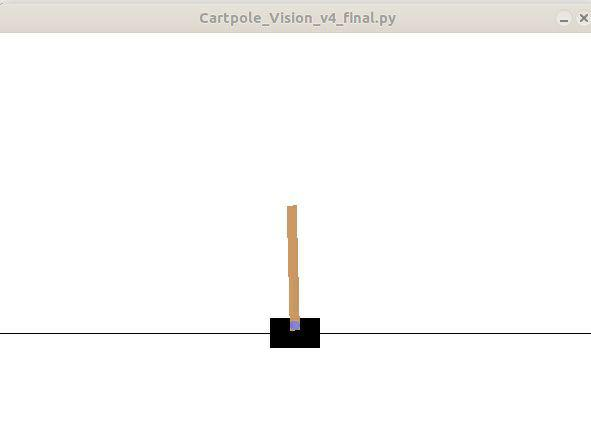
\includegraphics[width=12cm]{images/Cartpole_screenshot.jpg}
	\caption{Screenshot of the CartPole environment}
	\label{fig:CartPoleScreenshot}
\end{figure}

In the discrete version, it has a four dimensional observation space of the cart position, cart velocity, pole angle, and pole angular velocity as shown in Table \ref{table:tableenvironment}.

\begin{table}[h!]
	\centering
	\begin{tabular}{ |p{2cm}|p{4cm}|p{2cm}|p{2cm}|  }
		\hline
		\multicolumn{4}{|c|}{Observation Space} \\
		\hline
		Num & Observation & Min & Max \\
		\hline
		0 & Cart Position & -2.4 & 2.4 \\
		1 & Cart Velocity & $-\infty$ & $+\infty$ \\
		2 & Pole Angle & $\-41.8$\textdegree & $41.8$\textdegree \\
		3 & Pole Angular Velocity & $-\infty$ & $\infty$ \\
		\hline
	\end{tabular}
	\label{table:tableenvironment}
	\caption{Table showing the CartPole's observation space}
\end{table}

 The available actions are two discrete ones: push left and push the cart right. The reward is defined as +1 for every time step the CartPole stands including the termination step. The task is considered achieved when the average reward of the last 100 episodes reaches a score of 195 over a maximum score of 200. Episode termination occurs when:

\begin{itemize}
	\item The pole angle is more than $\pm 12$\textdegree
	\item The cart position is more than $\pm 2.4$ (i.e. the center of the cart almost reaches the edge of the display)
	\item The episode length is greater than 200
  \end{itemize}

\section{Solving the Sensor-Based CartPole}
\label{sec:simpleCartPole}
The simplified CartPole version includes, as we have already seen, a bunch of state inputs which can be regarded as coming from sensors mounted on the CartPole. This task is actually relatively easy and it has been solved several times by both amateurs and researchers.
\\
\indent The solution with the DQN architecture consists of a neural network mapping the four-dimensional state to two output values as shown in Figure \ref{fig:easyDQN}\footnote{Source: \href{https://ferdinand-muetsch.de/CartPole-with-a-deep-q-network.html}{ferdinand-muetsch.de}}.

\begin{figure}[h!]
	\centering
	\label{fig:easyDQN}
	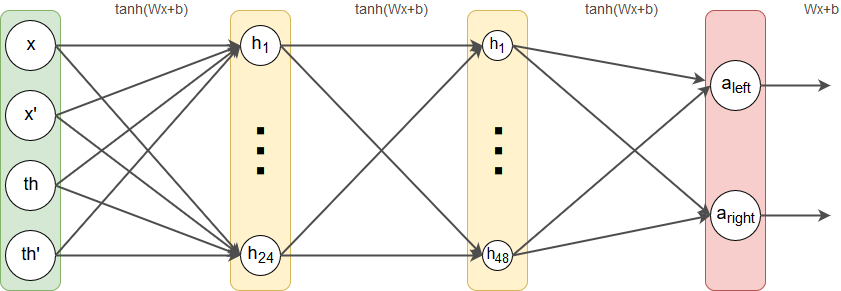
\includegraphics[width=12cm]{images/easycartpoleNN.png}	
	\caption{Neural network with four input neurons for the states, and two output neurons for predicting the actions values} 
\end{figure}

The two outputs give the state-action value of that particular action and the agent can select the action whose predicted value is the highest among the two actions. The architecture uses both an experience replay buffer, as explained in Algorithm \ref{alg:DQN} and the \textit{target network} for improving stability, as explained in Section \ref{sec:DDPG}. We have indeed two separate networks, one which is constantly being trained and a target network which is updated less frequently in order to decouple episode correlations and used in calculating the next state value. 
\\
\indent This DQN implementation shows great stability and is much faster than other algorithms like DDPG in solving the CartPole. Therefore, given that DQN is able to solve the low-dimensional CartPole and that working applications of DQN have been successfully implemented for complex tasks, we will make use of this algorithm for trying to successfully train an agent which can only see the environment's image and not its states.

\section{Towards Vision-Based Control}

The first steps in trying to solve the CartPole were based on a first implementation from Adam Paszke\footnote{\href{https://pytorch.org/tutorials/intermediate/reinforcement_q_learning.html}{Source: pytorch.org}}. The algorithm is based on Convolutional Neural Networks for predicting Q-values and implements basically the same structure of DQN described in Section \ref{sec:simpleCartPole}.
 
\begin{figure}[h!]
	\centering
	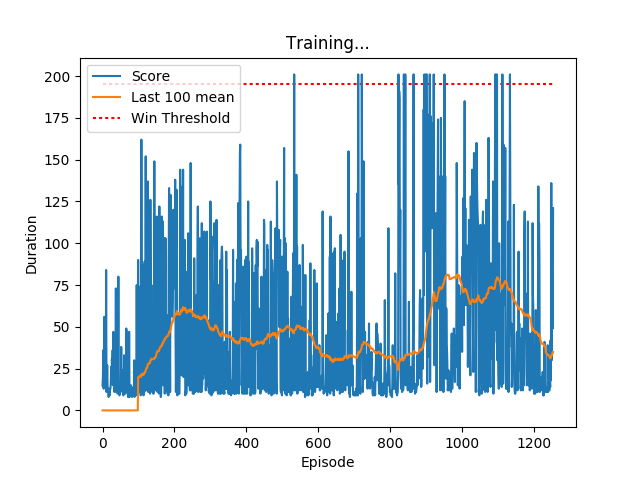
\includegraphics[width=14cm]{images/Vanishing_gradients.png}
	\caption{Oscillatory behavior of learning due to the vanishing gradients issue, showing no learning convergence. The orange line shows the mean of the last 100 episodes.}
	\label{fig:vanishingGradients}
\end{figure}

\indent The state observation is a cropped RGB image of the CartPole taken from its center. Since a single image would not be enough for capturing state change, since one single frame is static and cannot give any information about derivatives over time of position and angle (i.e. velocity and angular velocity), the difference between the current frame and the previous frame is taken as input. This is able to capture, at least at some degree, the cart and pole velocities.
\\
\indent However, no matter how much training the CartPole received, the mean reward was always swinging up and down and showing no sign of convergence or divergence as shown in Figure \ref{fig:vanishingGradients}. In particular, after some tenths of episodes showing an abrupt improvement in performance there were several episodes in which the CartPole seemed to "forget" about the previous experiences, suddenly decreasing the last 100 episodes mean required for solving the CartPole. Even changing the neural network's layers and tweaking hyper-parameters there was no sign of convergence in the algorithm.
\\
\indent After an extensive research, we have been able to find at least three major causes of this problem:

\begin{itemize}
	
		
	\item State observation: the state observation is a difference of cropped RGB images. However, better methods suitable for our CartPole environment observation exist and have proven profitable. 
	
	\item Overfitting: the network starts to learn filters and weights which allow the CartPole to stay in the upside position optimally. However, it has learned so well to stay in the upright position, that it basically "forgets" how to get there, hence starting a bunch of bad-scored episodes. When DQN returns negative feedback to these learned CNN parameters it starts again to learn, achieves a quasi-optimal behavior, and then fails again due to overfitting (see Section \ref{sec:overfitting}).
	
	\item Reward function: the reward function design is one of the crucial aspects of DRL agent design. In this case, the reward of just $\pm 1$ for each time step does not help the agent in any way to improve its stability: hence, changing the reward function can lead to robustness in the control system.

\end{itemize}

Thus, before showing the final algorithm specifications in section, we will first examine solutions to these two problems.

\subsection{Improving Image Pre-Processing}

One first step of state observation improvement implies simplifying the network by feeding it with a grayscale as input, thus reducing by one third the input dimensionality. Besides, the use of image subtraction may not work so well, since pixel-by-pixel difference can result in unwanted constructs such as negative valued pixels; indeed a better way to deal with changing environments over time is to feed the neural network a batch of images, them being the last N frames. This way, the state keeps track of past behaviors: if we just had one single frame at a time for predicting Q-values then the state would be non-Markovian (see Section \ref{sec:markov}). By considering at least the last $N=2$ frames, velocity features can be extracted by the neural network from the state.

\begin{figure}[h!]
	\label{fig:ExampleExtractScreen}
	\centering
	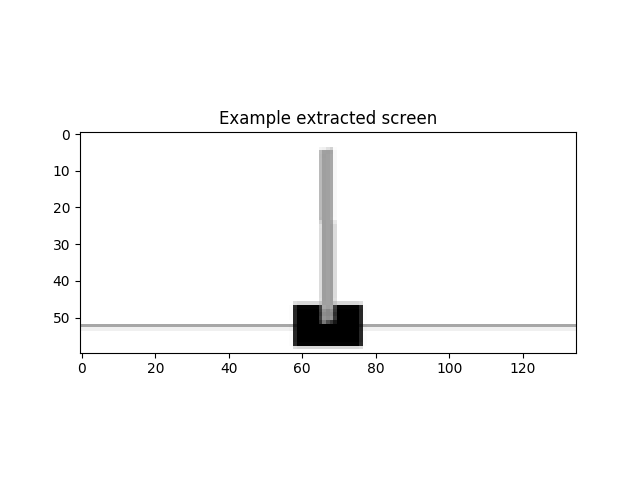
\includegraphics[width=12cm]{images/Example_extracted_screen.png}
	\caption{Extracted screen from the CartPole environment: the image is extracted by cropping, downsampling and applying grayscale. This is the only state input for the DQN algorithm.}
\end{figure}

\indent The image pre-processing resizes it and downsamples to a width times height value of 60x135, converted to grayscale as shown in Figure \ref{fig:ExampleExtractScreen}. The first observation cannot keep track of the previous frames, because there is no previous state: therefore, the same first frame is copied $N$ times in the frame buffer which is handled by a \textit{FIFO (First In First Out)} policy for updating it at each time step, thus keeping track of the $N-1$ previous frames. We set the image batch size $N=2$ based on empirical results which tell us this number of features makes the network converge faster.
\\
\indent This way, we obtain a total input dimension for the CNN, according to the PyTorch size\footnote{In PyTorch, images are represented as: \textit{[batch\_size, channels, height, width]}, where channels for RGB images are 3, and for grayscale one there is just 1 channel.}:

\begin{equation}
	\text{Image batch dimension} = [2, 1, 60, 135] = \text{2 x 1 x 60 x 135} = 16200
\end{equation}

As we can see, the dimensionality to be handled by the CNN is very high, and it would be almost impossible to use a simple feed-forward neural network.

\subsection{Dealing with Overfitting}

As regards the overfitting problem there are a couple of tweaks to prevent it from happening at all. First of all, we implement a \textit{Dropout}\footnote{Dropout\cite{srivastava2014dropout} is a method by which some neural network neurons are switched off during training with a probability $p_i$, hence "dropped-out". During the testing phase, all the neurons are switched on with their output multiplied by a weight $p_i$. This method has proven to make neural networks more stable and robust.} regularization for improving the network stability. However, this has little effect in the training process, because of the intrinsic problem of learning, forgetting and learning again.
\\
\indent Thus, another method we can use is that of the \textit{Early Stopping}: basically, in order to prevent overfitting,the agent is trained up to a point in which it has learned optimal behavior; from that point onward it would start behaving worse and worse and then restarting learning from scratch. We can detect this optimal situation by inserting a score threshold: when the mean of the last $K$ episodes overcome this threshold $\xi$, we stop the neural networks optimization. We have empirically set these two new hyper-parameters, which can be tweaked, to $K = 20$ and $\xi= 142$.


\subsection{Reward Function Design}
The reward function design is one of the aspects of paramount importance in Reinforcement Learning and can make the difference between an agent not training at all and one able to achieve super-human performance. Instead of the usual reward function $r$, we built a new one being able to better give a feedback on our agent's decisions:

\begin{equation}
\label{eq:reward}
\begin{aligned}
	r_1 = \frac{x_{max} - |x|}{x_{max}} - 0.8 \\
	r_2 = \frac{\theta_{max} - |\theta|}{\theta_{max}} - 0.5 \\
	r_{tot} = r_1 + r_2 
\end{aligned}
\end{equation}

Where $x$ is the CartPole position, and $\theta$ is its angular position. This reward function gives the highest reward when the CartPole is at the center of the screen, with no inclination and gives the worst reward to the CartPole being either at the screen edges or with the pole very inclined. Besides, we give a negative reward of $-20$ to actions making the episode end before reaching the 200 score and a positive reward of $+20$ to actions making the CartPole balance up to 200, thus penalizing bad actions and "encouraging" good ones.
\\
\indent We can assert from empirical results that this reward function design is able to better stabilize the CartPole, since it will try to reach the maximum reward by staying in the upright position with minimum displacement on the track. 

\section{Vision-Based Control}

After dealing with the major problems leading to oscillatory behavior of the reward, we finally present in this chapter the final setup for a successful implementation of the CartPole vision-based control. We firstly show the hyper-parameters setting for achieving the result and after that we will jump to the final results of the experimental setup.

\subsection{Convolutional Neural Network Design}

The Convolutional Neural Network parameters are shown in the Table \ref{table:NeuralNetwork}. The number of neurons in a Convolutional Layers is the number of filters that can be learned, while as for the Linear Layers it is the number of neurons itself as in the feed-forward networks described in Chapter \ref{sec:feedforward}. 
\\
\indent As regard the other two parameters, the \textit{kernel size} is the size of the square filter actuating convolution over the inputs (i.e. in our implementation we have a 5x5 filter). The second parameter, the \textit{stride}, is the number of pixels which are "skipped" each time while making the filter convolve. A higher stride will make the model less precise, but slower in learning; a $stride = 2$ is usually chosen because has been empirically proven to be the best choice for CNNs.


\begin{table}[h!]
	\centering
	\begin{tabular}{ |p{4cm}|p{3cm}|p{2cm}|p{1.5cm}|p{1.2cm}|  }
		\hline
		\multicolumn{5}{|c|}{Neural Network Parameters} \\
		\hline
		Layer & Number of Neurons & Activation & Kernel Size & Stride \\
		\hline
		Convolutional Layer 1 & 16 & ReLu & 5 & 2\\
		\hline
		Convolutional Layer 2 & 32 & ReLu & 5 & 2 \\
		\hline
		Convolutional Layer 3 & 32 & ReLu & 5 & 2 \\
		\hline
		Linear Output Layer  & 1792 & None & - & - \\
		\hline
	\end{tabular}
	\label{table:NeuralNetwork}
	\caption{Convolutional Neural Network hyper-parameters}
\end{table}
	
Other important settings for the CNN are the following:

\begin{itemize}
	\item Loss Function: \textit{Huber loss function}, which is: 
	\begin{equation}
		L(Q_{target}, Q_{predicted}) = \frac{1}{2}(Q_{target}-Q_{predicted})^2
	\end{equation}
	\item Optimizer: \textit{RMSprop}, which is able to do a gradient descent of the error in almost the most optimal path
\end{itemize}

\subsection{Hyper-Parameters Settings}

In Table \ref{table:hyperParameters} the main DRL Hyper-Parameters are summarized, based on the DQN with Experience Replay and Target Network of \ref{sec:DQN}.


\begin{table}[h!]
	\centering
	\begin{tabular}{ |p{6cm}|p{6cm}| }
		\hline
		\multicolumn{2}{|c|}{Hyper-Parameters Values} \\
		\hline
		Batch Size & 128 \\
		\hline
		Batch of Frames Size & 2 \\
		\hline
		Discount Rate $\gamma$  & 0.999 \\
		\hline
		Initial $\varepsilon$ & 0.9 \\
		\hline
		Final $\varepsilon$ & 0.05 \\
		\hline
		$\varepsilon$-Decay & 5000 \\
		\hline
		Early Stop $\xi$ & 142 \\
		\hline
		Image Height (pixels) & 60 \\
		\hline
		Image Width (pixels) & 135 \\
		\hline
		Maximum Memory Size  & 100000 \\
		\hline
       	Target Model Update $\tau$ & 50  \\
        \hline

	\end{tabular}
	\label{table:hyperParameters}
	\caption{Reinforcement Learning hyper-parameters}
\end{table}

The exploration and exploitation problem described in Section \ref{sec:explorationExploitation} is dealt with by the use of the following $\varepsilon_{threshold}$:

\begin{equation}
	\varepsilon_{threshold} = \varepsilon_{final} + (\varepsilon_{initial}-\varepsilon_{final})e^{-t/\varepsilon_{decay}}
\end{equation}

In order to obtain an $\varepsilon$-greedy policy in Python, we use a uniformly random generator of numbers $\in[0,1]$. Then, if the generated number is greater than the $\varepsilon_{threshold}$ the action selection will be greedy, otherwise it will select a random action. In this way, it is possible to obtain a good compromise between exploration and exploitation of the CartPole agent.

\subsection{Final Results}

After several unsuccessful or partially successful tries, using a tweaked CNN architecture, regulated Hyper-Parameters and adjustments in image pre-processing, dealing with overfitting and reward function design, we finally come to the experimental results.
\\
\indent In the experimental tests, many episodes were run to see how was the behavior of the CartPole under our new design. As it can be noted from Figure \ref{fig:CartPoleWon} we were able to reach our final result: stabilizing a cart and pole system with only vision-based input for control feedback.\footnote{The algorithm can be found at this \href{https://github.com/fedebberto/Vision_Based_CartPole_DQN}{Federico Berto's Github repository}.}

\begin{figure}[h!]
	\centering
	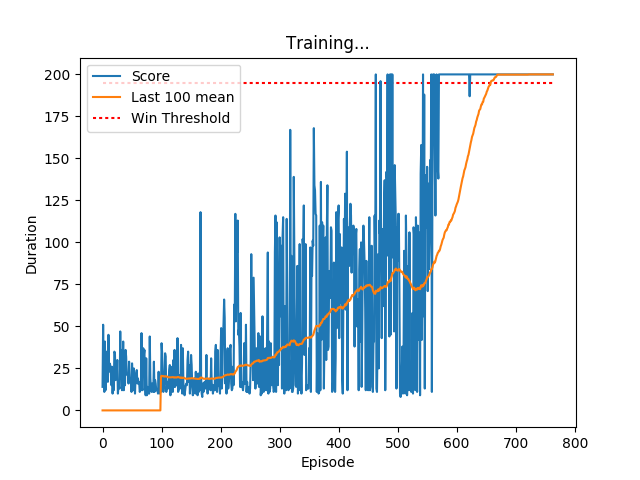
\includegraphics[width=14cm]{images/Cartpole_vision_beaten@659_reached_perf@723.png}
	\caption{Graph showing CartPole balancing score with respect to an over 800 episodes time span, with training beginning from scratch. Winning has been achieved at episode 659, scoring more than the 195 mean reward over the last 100 episodes required for success. At episode 723, the average reward of 200/200 was reached in this training session.}
	\label{fig:CartPoleWon}
\end{figure}

The results showed convergence in a real-time training session of around $10\sim15$ minutes with our not-state-of-the-art PC with specifications described in Section \ref{sec:hardwaresoftware}. 
As the graph shows, the Vision-Based CartPole manages to reach the last 100 episodes mean of 195/200 in generally about $500\sim700$ episodes, thus officially beating the original OpenAI Gym's game with an even much more challenging input state.


\chapter{Conclusions and Future Work}
\label{ch:conclusion}

In this final chapter we summarize our research and experimental implementations and also give some ideas for possible improvements and further work.

\section{Thesis Summary}

The goals of this thesis were to provide the reader with a useful introduction to the Reinforcement Learning research field and to demonstrate the abilities of Deep Reinforcement Learning in achieving vision-based control.
\\
\indent We briefly presented the main three branches of Machine Learning among which Reinforcement Learning is. After that, we have presented the bases of the theory behind RL which is nowadays a very lively research field and is very attractive because of its possible implementations in not only control theory but also in many other fields.
\\
\indent We explained the main concepts of SARSA, Q-Learning, the Actor-Critic Methods and the Deterministic Policy Gradients and gave a brief introduction of model-based ones. The main problem of these methods was that they would require a huge amount of memory since they store value functions in a tabular form, hence function approximators are used for such tasks.
\\
\indent The most robust and used function approximators are nowadays Neural Networks. NNs are able to approximate functions by means of storing information in weights; these are able to create a network which is updated to approximate in the best way possible a function relating inputs to outputs. A particular implementation is the Convolutional Neural Network, which is the base of vision-based function approximation.
\\
\indent Deep Reinforcement Learning, whose most notable algorithms which are presented are DQN, DDPG and TRPO, combines classical RL algorithms with the power of Neural Networks making otherwise impossible tasks solvable. DRL has made huge progress in recent years, proving that it is possible to train agents dealing with highly challenging tasks.
\\
\indent The experimental part is made to demonstrate the power of DQN in stabilizing one of the benchmarks of DRL algorithms, the CartPole. We made a further step in developing an implementation able to achieve vision-based control of the system, a much more challenging task compared to the classical problem. After many unsuccessful experiments, we were able to solve the problem making the algorithm fail, mainly due to image pre-processing, overfitting and reward function design. We designed a Convolutional Neural Network for approximating image frames to their values and implemented DQN: the final results were very satisfactory in showing the CartPole stabilization and beating the OpenAI's challenge.

\section{Future Work}

In this section some further advice for possible future work is given to the reader.
\\
\indent Fist of all, the Deep Reinforcement Learning research field is very active and each year a number of research papers are released, some of them containing new algorithms and methods for solving a wide variety of tasks. Up to now, no DRL method can be said to be perfect since some methods which excel in a task may not be able to solve another one and vice-versa; thus, fresh research of the new and most recent evolution of this ever-changing research field should be done.
\\
\indent As regards the experimental part, the vision-based CartPole algorithm can be further improved. For example, an improvement may be making it able to beat the \textit{"CartPole\_v1"} version of OpenAI Gym which raises the win threshold to 500, hence making the algorithm more stable. Moreover, DQN itself may not be the perfect choice for the CartPole: for instance, TRPO has proven a much more robust though complex algorithm in a wide variety of tasks.
\\
\indent Besides the main thesis body, Appendix \ref{appendixA} and Appendix \ref{appendixB} are provided to the reader for a more comprehensive introduction to RL. The former explores further Reinforcement Learning algorithms while the latter explains and evaluates the main state-of-the-art advances in Deep RL as of the time of writing (2019).
\\
\indent Another advice for the reader is also that interesting implementations include more sophisticated and complex environments such as the Atari Arcade platforms or the 3D simulation MuJoCo environment. An even more appealing goal would also be being able to implement Reinforcement Learning on a real world task which is indeed the ultimate goal of RL: enabling machines to learn and make decisions in our world.

\appendix

\chapter{Additional Reinforcement Learning Algorithms}
\label{appendixA}

\section{Model-Free Methods}
In this section we will explore more advanced model-free methods and concepts which may be useful for the reader in order to develop more advanced implementations of Reinforcement Learning. 

\subsection{TD($\lambda$)}
It is clear that one of the most important differences between the Monte Carlo methods and TD ones is that, while the former use a total reward for value function update, the latter use rewards at the current step. A way to combine both approaches would be to use the returns obtained after every certain number of steps, instead of taking the total returns after each episode, and then calculating a weighted average of them: this is the main idea behind the TD($\lambda$) algorithm.
\\
\indent The "$\lambda$" stands indeed for an additional variable associated to each state, known as \textit{eligibility trace} $e_t(s) \in \mathbb{R}^+$. The eligibility trace indicates how much learning should be assigned to each state at every time step, depending on the frequency and recency of the visit for each state. Eligibility traces are updated at each time step using the following rule: 

\begin{equation}
e_t(s) = \begin{cases}
\gamma\lambda e_{t-1}(s), & \text{if $s \neq s_t$} 
\\
\gamma\lambda e_{t-1}(s) +1, & \text{if $s = s_t$} 
\end{cases}
\end{equation}

where $\lambda$ is known as the \textit{trace-decay parameter}. This is referred to as the \textit{accumulating} form of the eligibility trace, because every time a given state is encountered the trace is incremented by one; the more a situation occurs over time, the more it is kept track of with this method.
\\
\indent The value function is then updated, for instance using SARSA or Q-Learning update, weighted by eligibility traces. The Q-Learning algorithm we have analyzed before actually employs a particular version of the TD($\lambda$) algorithm, which is the TD(0): by fixing $\lambda = 0$, only the latest state encountered counts for the value function update. If $\lambda = 1$, the result is practically the same as in Monte Carlo updates. By properly choosing a value of $\lambda$ between 0 and 1, we can give the algorithm positive features from both Temporal Difference Learning and Monte Carlo.

\subsection{Policy Search Methods}

Policy search methods are a class of RL algorithms using parametrized policies $\pi_{\theta^\pi}$, with $\theta^\pi$ being the parameter vector. These methods search in the parameter space $\Theta$, a $\theta^\pi \in \Theta$ for an optimal policy. Policy evaluation occurs by performing rollouts from the current policy and calculating the total reward. Then, parameters are updated using gradient ascent in the direction of increasing expected return, hence improving the policy by making the total rewards increase. The update rule for the parameters of the policy can be expressed in terms of J, the expected return, as:

\begin{equation}
	\theta_{t+1}^\pi = \theta_t^\pi + \alpha \nabla_{\theta^\pi}
\end{equation}

where,

\begin{equation}
	J = \mathbb{E}_\pi (\sum_{k=0}^{\infty}\gamma^kr_k)
\end{equation}

As for how the gradient is defined and evaluated, there is a wide variety of policy search approaches we are not going to discuss into detail here.
\\
\indent In contrast with value based approaches, policy search ones have better convergence properties and can also learn stochastic policies . However, the major drawback of these algorithms is their policy evaluation step, suffering from great variance and thus making learning slow. This means that a large number of interactions is needed, making it undesirable for tasks involving real world robots. Methods to overcome these challenges include pre-structured policies, such as motor primitives, %(CITATION NEEDED)
and additional information for bootstrapping policy parameters, such as human demonstration, thus leading to faster convergence.

\subsection{Actor Critic Methods}
\label{sec:actorcritic}

Actor critic methods\cite{konda2000actor} are TD methods which store the policy explicitly. Since the policy chooses actions in a given state, it is known as the \textit{actor}, while the value function acts as the \textit{critic} constantly evaluating the policy based on the temporal difference error. The policy itself is updated based on the critic. 
\\
\indent Policy updates are similar to policy search methods, except that the critic decides the direction of gradient ascent instead of the expected return: this helps reducing the variance for these types of algorithms. The stochastic policy gradient theorem defines J, the gradient of the expected return, as:


%NEW LINE FOR EQUATION + TILDES

\begin{align}
	\begin{split}
		\nabla_{\theta^\pi}J &= \int_{\textbf{S}}\rho_\pi(s) \int_{\textbf{A}} \nabla_{\theta^\pi} \pi (a|s; \theta^\pi)Q(s, a; \theta_Q)dads \\
		&	= \mathbb{E}_{s\sim\rho_\pi, a\sim\pi(a|s; \theta^\pi)} [\nabla_{\theta^\pi} \pi(a|s; \theta^\pi)Q(s,a; \theta^Q)]
	\end{split} 
\end{align}

where $\rho_\pi(s)$ is the state distribution under policy $\pi$, $\theta^\pi$ is the parameter vector for the policy $\pi$ and $\theta^Q$ is the parameter vector for Q-function. The parameters of the value function, $Q(s, a; \theta^Q)$, are updated using temporal difference learning. These algorithms are known as \textit{stochastic actor critic algorithms}.

\subsection{Deterministic Policy Gradient}
 A deterministic counterpart to the stochastic actor critic methods, known as \textit{Deterministic Policy Gradient (DPG)} has been introduced in literature for the expected return $J$ when subject to a deterministic policy. In this case, the gradient for the expected return can be written as:

\begin{align}
\label{eq:DPG}
	\begin{split}
		\nabla_{\theta^\pi}J &= \int_{\textbf{S}}\rho_\pi(s) \nabla_{\theta^\pi} \pi (s; \theta^\pi) \nabla_a Q(s, a; \theta_Q)|_{a=\pi(s, \theta^\pi)}ds \\
		 &= \mathbb{E}_{s\sim\rho_\pi} [\nabla_{\theta^\pi} \pi(s; \theta^\pi)\nabla_a Q(s,a; \theta^Q)|_{a=\pi(s, \theta^\pi)}] 	 
	\end{split}
\end{align}

 Since there is a continuous feedback loop of the actor and critic, actor critic methods are mostly on-policy. However, off-line counterparts have been introduced in literature.
\\
\indent Actor critic methods provide better convergence properties than the previous TD ones, and they also make action computation easier, especially for continuous tasks. Besides, they can also learn stochastic policies. However, since tabular methods are not implementable for high dimensionality state and action spaces, we are required to implement a further piece using function approximators, such as neural networks, for obtaining satisfactory real life results.

\section{Model-based Methods}

All the approaches we have discussed up to now do not possess any previous knowledge of the environment, thus they are called \textit{model-free methods}. Model-based methods try to utilize some information about the environment in order to speed-up the learning process.
\\
\indent There are basically two approaches in model-based learning: one is to build a model of the environment from first principles and then use it to learn the policy or value function. The other approach is to learn a model of the environment by experimenting on it. The problem with the former approach is that, if the model is not that accurate, then the learned policy will likely be sub-optimal, or even fail in learning anything at all. Therefore, most successful model-based approaches actually try learning a model and using that to speed up learning.	
\\
\indent A variety of forward models %INSERT LITERATURE
have been proposed in literature for planning: locally linear models, Gaussian Process models, DNN and so on. However, since the purpose of this thesis is to provide a preliminary study on RL and it is going to focus more on model-free methods, we are not going to deep-dive into model based ones, although we have provided a general idea for the sake of clarity.



\chapter{Additional Deep Reinforcement Learning Algorithms}
\label{appendixB}

\section{Deep Deterministic Policy Gradient}
\label{sec:DDPG}
Deep Deterministic Policy Gradient (DDPG)\cite{lillicrap2015continuous} derives from the actor-critic framework discussed in Section \ref{sec:actorcritic} and it provides an improvement with respect to the DQN discussed above by making it tractable for continuous actions spaces. In DDPG, the actor is described by a neural network and the critic by another one. As the name suggests, the update rule for the value is the same one as for the Deterministic Policy Gradients in Equation \ref{eq:DPG}. This is also an off-policy algorithm.
\\
\indent In DQN, we have observed that directly updating networks by taking the temporal difference error could result in divergence sometimes. DDPG introduces a couple of improvements over traditional actor-critic in order to make learning suitable with neural networks: the first one, which was already used in DQN is the \textit{experience replay}, and the other one is the use of \textit{target networks}.Target networks are basically copies of the actor and critic networks: they are used to calculate the target $y$ for the temporal difference error. The target networks are updated very slowly to track the learned networks: learning the optimal Q-function becomes a supervised learning problem which stabilizes the algorithm greatly.
\\
\indent The update for the critic is given by the standard Q-learning update of Equation \ref{eq:gradientloss} by taking targets $y$ to be:

\begin{equation}
	\label{eq:criticupdate}
	y = \mathbb{E}_{s'\sim\epsilon}[r + \gamma Q'(s', \mu'(s'; \theta^{\mu'})\theta^{Q'})]
\end{equation}

where $Q'(s, a; \theta^{Q'})$ and $ \mu'(s; \theta^{\mu'})$ refer to the target networks for the critic and the actor respectively with weights $\theta^{Q'}$ and $\theta^{\mu'}$.
\\
\indent The loss function is defined as:

\begin{equation}
	\label{eq:lossactorcritic}
	L = \mathbb{E}_{s\sim\rho_\beta, a\sim\beta}\left(y-Q(s,a; \theta^Q)\right)^2
\end{equation}

where $Q(s, a; \theta^Q)$ refer to the critic network with weights $\theta^Q$ and $\beta$ is the behavior policy.
\\
\indent The policy is updated using the DPG theorem from Equation \ref{eq:DPG} given by:

\begin{equation}
	\label{eq:DPG_actorcritic_gradient}
	\nabla_{theta^\mu}J = \mathbb{E}_{s_\sim\rho_\beta}[\nabla_aQ(s, a; \theta^Q)|_{s, a=\mu(s;\theta^\mu)}\nabla_{\theta^\mu}\mu(s; \theta^\mu)|s]
\end{equation}

where $\mu(s; \theta^\mu)$ refers to the actor with weights $\theta^\mu$.
\\
\indent The complete DDPG algorithm written in pseudo-code Algorithm \ref{alg:DDPG} is given below:

\begin{algorithm}[h!]
	\caption{Deep Deterministic Policy Gradient}
	\label{alg:DDPG}
	\SetAlgoLined
	\DontPrintSemicolon
	Initialize replay memory $\mathcal{D}$ \;
	Initialize critic network $Q$ and actor network $\mu$ with random weights $\theta^Q$ and $\theta^\mu$ respectively \;
	Initialize target networks $Q'$ and $\mu'$ with weights $\theta^{Q'} \leftarrow \theta^Q$, $\theta^{\mu'} \leftarrow \theta^\mu$
	\Repeat{terminated}{
		Observe initial state $s_1$\;
		\For{t=1: T}{
			Select an action $a_t = \mu(s_t; \theta^\mu) + \mathcal{N}$\;
			Carry out action $a_t$\;
			Observe reward $r_t$ and new state $s_{t+1}$\;
			Store transition $(s_t, a_t, r_t, s_{t+1})$ in replay buffer $\mathcal{D}$\;
			Sample random transitions from $\mathcal{D}$\;
			Calculate target for each transition using \ref{eq:criticupdate}\;
			Train the critic network using stochastic gradient descent by minimizing \ref{eq:lossactorcritic}\;
			Update actor network using \ref{eq:DPG_actorcritic_gradient} \;
			Update the target network using 
			% MATCH SYNTAXXX!! LIKE s'
			\begin{equation}
				\begin{aligned}		
				\theta^{Q'} \leftarrow \tau\theta^Q + (1-\tau)\theta^{Q'}
			\\
			\theta^{\mu'} \leftarrow \tau\theta^\mu + (1-\tau)\theta^{\mu'}
				\end{aligned}
			\end{equation}
		}
	}
\end{algorithm}



\section{Trust Region Policy Optimization}
Trust Region Policy Optimization (TRPO)\cite{schulman2015trust} works by minimizing a certain objective function, ensuring monotonic improvements for the policy. It builds up on policy gradient methods addressing one of their most important issues: the bad choices made by the optimizer which usually does not work very well in curved areas, hence ruining the progress. An analogy for this problem can be found in learning how to follow a mountain path: if the agent were overconfident of its progress, then it could make a bad decision in following the steepest gradient ascent by making a line step directly down a cliff, ruining the progress and possibly damaging itself in a real-world scenario instead of following the path in a more cautious way. TRPO chooses a radius $\delta$ giving an area in which to look for the best value instead of naively following a line path for the gradient ascent: this is called the trust region. This way, we have a constrained optimization problem which can be stated as:


\begin{equation}
\label{eq:TRPO}
	\begin{aligned}
		\max_{\theta^\pi}\mathbb{E}_{s\sim\rho_{\pi(\cdot)}, a\sim\pi_{(\cdot;\theta^\pi_i)}} \left( \frac{\pi(a|s; \theta^\pi)}{\pi(a|s; \theta^\pi_i)}Q_\pi(s,a) \right) \\
		\text{subject to $\mathbb{E}_{s \sim \rho_{\pi(\cdot)}}$} \big(D_{KL}		\pi(\cdot|s;\theta^\pi_i)||\pi(\cdot|s;\theta^\pi)\big) \leq  \delta 
	\end{aligned}
\end{equation}


where $\pi(a|s; \theta^\pi_i)$ denotes the policy at iteration $i$ $\rho_{\pi(\cdot)}$ denotes the state visitation frequency under policy $\pi_{\theta^\pi_i}$ and $\delta$ is the step size which decides how much the new policy is allowed to deviate as compare to the old policy. $D_{KL}$ indicates instead the Kullback–Leibler divergence\footnote{The Kullback-Leibler divergence (which can be found in full form at \cite{hershey2007approximating}, is a measure of how a probability distribution differs from another. In other words, TRPO puts a limit to this difference bounding it in a "safety" radius $\delta$, the trust region. }.
\\
\indent TRPO has demonstrated robust performance in a wide variety of tasks such as walking, swimming and hopping gaits. The algorithm has a performance which is similar to the DQN algorithm (Section \ref{sec:DQN}) on the Atari games domain, hence making it one of the most robust and adaptable Deep RL algorithms.

\section{Other Deep RL Algorithms}

More advanced Deep Reinforcement Learning algorithms generally build up on the ones we have analyzed up to now and since RL is a continuously developing research subject, many new algorithms and improved variants are being developed as the time of writing. As we have seen with the DDPG and TRPO, the most challenging tasks,  are the high-dimensional ones. 

\subsection{Generalized Advantage Estimation}
Generalized Advantage Estimation (GAE)\cite{schulman2015high} builds on the TRPO and its aim is to solve the issue of the latter, which is requiring a large number of samples for policy improvement. Instead of using the Q-function in Equation \ref{eq:TRPO}, GAE uses an exponentially weighted estimate of the advantage function, which we are not going to discuss, for reducing estimates variance of policy gradients. 
\\
\indent The algorithm has proven able to solve highly challenging tasks such as 3D locomotion ones, which are high-dimensional in both states and actions spaces.

\subsection{Guided Policy Search}
Guided Policy Search (GPS)\cite{levine2013guided} implements a different approach with respect to the methods shown before. The method has been used to learn neural network policies for high dimensional tasks and has proven extremely sample efficient, which is critical for tasks involving real robots.
\\
\indent The main idea of GPS is to first do a trajectory optimization for the given task and learn an optimal distribution over trajectories: after that, the samples from our optimal distribution are used to train via supervised learning a neural network policy. In other words, we are using a demonstration of the optimal policy and then using that to bootstrap and speed-up the learning process making it more sample efficient.
\\
\indent In the trajectory optimization stage we are using a full knowledge of the system: thus, this is a form of \textit{instrumented training}. Other than using demonstration, for instance by a human, for reducing the sample complexity we can further improve the sample efficiency by pre-training the neural network to predict certain elements of the state space which are not observable. GPS is able to speed learning up by actually having a teacher: it builds up on the idea that, having someone or something to learn a task from, will make the learning process easier and faster as it happens in the real world with animals and human beings.

\section{Deep RL Algorithms Comparison}

We will now compare the DRL algorithms shown in the sections above based on 4 different criteria:

\begin{itemize}
	
	\item Ability to learn from off policy data: this criterion is important because it allows the agent to learn from previous experience which can first be collected and used after. Both DQN and DDPG can learn from off-policy data since they use a replay buffer. Policy gradient methods and GPS, on the other hand, require on-policy data to train the network.
	
	\item Robustness: TRPO and the model-based TRPO-GAE and GPS are more robust since their policy optimization procedure guarantees a monotonic improvement.
	
	\item Sample Efficiency: GPS is the most sample efficient, being a model-based algorithm which utilizes trajectory optimization along with neural network training.
	
	\item Scalability: All of the DRL methods, apart from DQN, have shown that they can be applied on continuous high dimensional tasks.

	
\end{itemize}


\newpage


\bibliographystyle{ieetr}
\nocite{*}
\bibliography{chapters/bibliography}








\end{document}